%%%%%%%%%%%%%%%%%%%%%%%%%%%%%%%%%%%%%%%%%%%%%%
\logvartrue
\chapter{Introduction}
%%%%%%%%%%%%%%%%%%%%%%%%%%%%%%%%%%%%%%%%%%%%%%

The past century has seen a series of important steps forward in many fields of science, never experienced before in the recent history of mankind: the basis posed by illuminism and the industrial revolution in the 19th century have bloomed in the 20th century, with a prominent role of science in translating theoretical insights into broadly adopted technological advances. One of the fields that has been pushed forward the most is biology, in which the brilliant ideas of pioneers like Charles Darwin \cite{darwin1869origin} and Gregor Mendel \cite{mendel1865experiments} have formed the basis for the modern views in the function and evolution of all life forms. In particular, the depiction of the molecular basis of cell biology, proposing a central role of the genetic material as the repository of the functional and evolutive information, has lead to the development of a series of fields of biology devoted to the study of the interaction between this genetic material (\textit{genotype}) and the cell behaviour (\textit{phenotype}).  

\section{The genomics era: from genes to genomes}
For a long time since its first definition (1909), the gene has been recognized as the atomic component of the genetic material, more than 30 years before the final proof that DNA was the repository of the genetic material; during the following fifty years further discoveries had unraveled the mechanisms with which the genetic material is translated into proteins (and therefore functions and phenotypes), defining the genetic code, the central dogma of biology and the mechanisms of genetic evolution through mutational events at the nucleotide level. All this concepts focus on a new atomic element that is the genetic sequence, which is simply a series of ordered and sequential nucleotides that contain both the genes and all the other regulatory elements; as a consequence of this consideration, a strong effort in the scientific community has been focused in creating technologies that would have made possible to read these sequences.

\begin{figure}[!tb]
	\center
    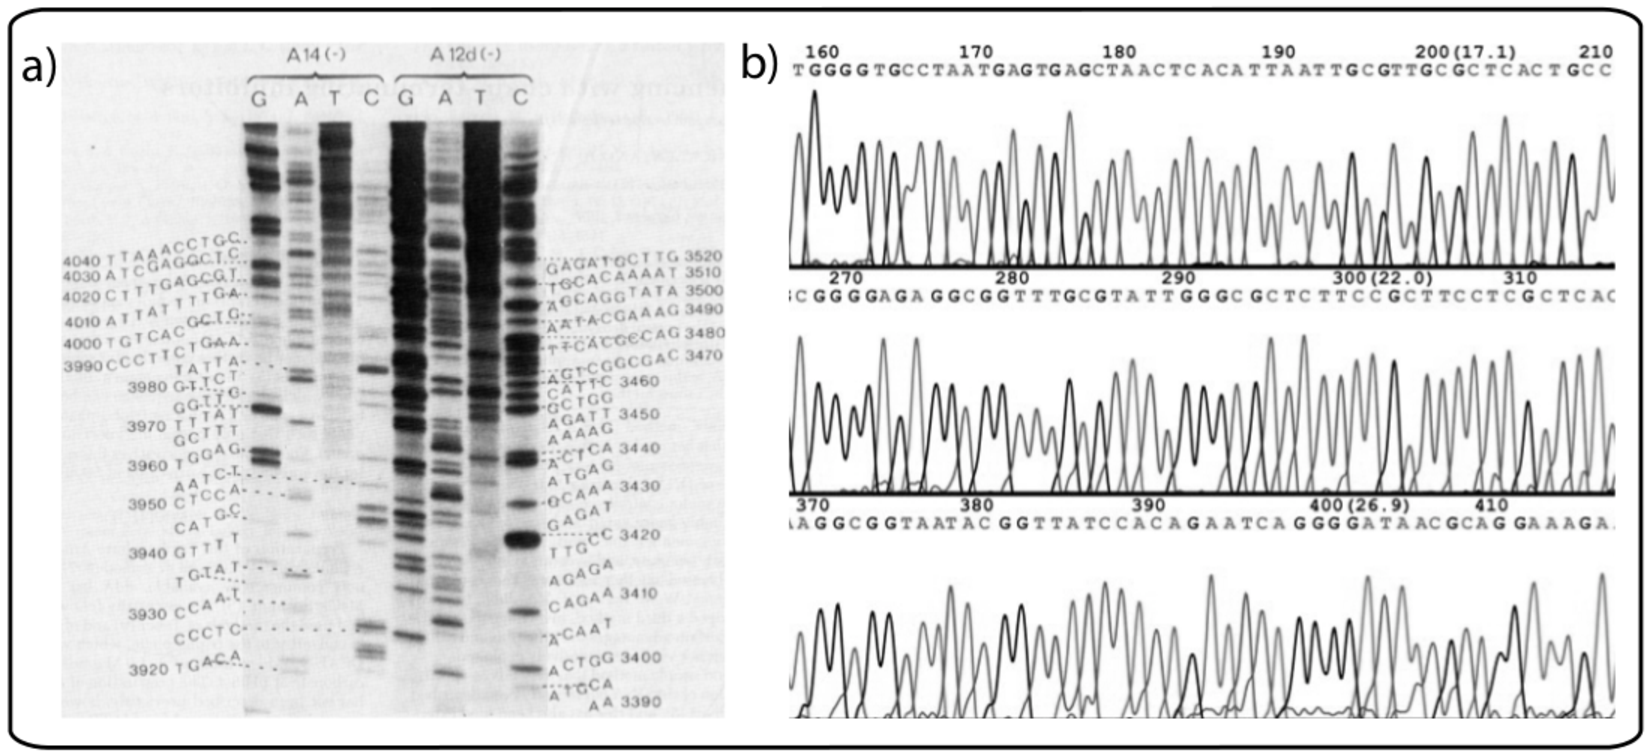
\includegraphics[width=1\textwidth]{figures/Introduction/thesis_1}
	\caption{\label{fig:sanger}\textbf{Evolution of Sanger sequencing}\\
			a) Autoradiograph of an acrylamide gel \cite{sanger1977dna} \\
			b) Electropherogram of a dye terminator sequencing, separated by capillar electrophoresis \cite{electropherogram}}
\end{figure}

The first method to be successfully adopted for DNA sequencing was developed by Sanger and colleagues (\cite{Sanger1975441} and \cite{sanger1977dna}) and is known as chain-termination sequencing: the single strand template is replicated using the enzyme DNA-polymerase and a set of nucleotides containing a certain amount of dideoxynucleotidetriphosphates (ddNTPs), which cause a termination in the DNA synthesis. During the next 40 years this technique has been refined, changing from the initial manual procedure using four different reactions with radioactive-labeled ddNTPs and a gel electrophoresis to the dye-terminator technology, in which the ddNTPs are labeled with a different fluorescent dye and the resulting fragments are separated by capillary electrophoresis and read with a laser (Figure \ref{fig:sanger}): this advances lead to the automation of the whole sequencing process, with a drop in cost and time needed. Thanks to this technological advances, it was no longer impossible to obtain the complete DNA sequence of an organism, at any phylogenetic scale: in fact, even if the first genomic sequences belonged to viruses \cite{sanger1978nucleotide} and small bacteria \cite{fleischmann1995whole}, the important contribution of computational techniques of the young field of bioinformatics helped in obtaining the genomic sequences of higher organisms such as yeast (\textit{Saccharomices cerevisiae}, \cite{goffeau1996life}), the nematode \textit{Caenorhabditis elegans} \cite{caenorhabditis1998genome}, the fruit fly (\textit{Drosophila melanogaster}, \cite{adams2000genome}) and of course the human genome (\cite{lander2001initial} and \cite{venter2001sequence}).

If this shift from a gene-centric to a genome-centric perspective made possible to study the whole repertoire of the genetic elements present in a given species, on the other hand a new challenge was immediately posed: the growing quantity of data produced (i.e. sequences) needed to be handled properly, since each fragment that is sequenced has a limited length and therefore needs to be tied together, and the genetic features have to be found inside the sequence. To overcome this new challenges that arose with the new sequencing technologies, the field of bioinformatics (also known as computational biology) was born: the biological sequences could then be encoded in a computer-friendly way and a series of algorithms that model biological processes could be created and applied to these sequences.

\subsection{From raw sequences to predicted functions}
In order to obtain a complete genome sequence of an organism, including the information regarding the position and function of each gene, a number of computational steps have to be applied, each one with different problems and constraints: with the evolution of sequencing technologies, the number of algorithms and softwares designed to address each one of the steps needed to obtain an annotated genomic sequence has increased.

\subsubsection*{Sequence trimming}
The first step in the sequence management directly involves the reads produces by the sequencing machine, which are short sequence fragments, and which strongly influences the following steps; disregard of the detection technology, each position is assigned to a base with an error probability. Since the sequence quality usually drops towards the read's end, it is important to remove the bases with higher error probability from the end of the sequence read, in order to ensure an accurate sequence; this process is known as \textit{trimming}. Trimming methods mostly rely on a particular quality encoding defined by the Phred program \cite{ewing1998base}\cite{ewing1998base2}, in which the quality score is logarithmically proportional to the base-call error probability (Equation \ref{eq:phred}); this quality measure has been encoded as ASCII characters together with the putative sequence in the FASTQ file format \cite{cock2010sanger}. 

\begin{equation}
\label{eq:phred}
Q = -10 \log_{10}P
\end{equation}

Usually a window approach is used to scan each read and discard those regions with poor quality (usually with Phred quality 30 or below, which corresponds to a base call accuracy of 99\%).

\subsubsection*{Assembly}
\label{sec:hamiltonian}
Once that the reads have been trimmed to remove low quality bases, the next task is to merge the short reads into larger sequences, which possibly can lead to reconstruct the whole target genome: the process is called \textit{assembly}; the adopted strategy strongly depends on the reads length, on the number of repetitions and sequence coverage, which can vary with each genome; in this paragraph only the approach used in sanger sequencing project is considered: the other algorithms will be discussed in section \ref{sec:revolution}. The core of each algorithm developed to assembly Sanger sequences relies on the measure of overlaps between the reads and the construction of a directed graph in which the nodes represent each read and the edges alignments between reads passing an arbitrary set of cut-offs: the final sequence is then reconstructed by looking for an Hamiltonian cycle inside this directed graph (Figure \ref{fig:assembly}) \cite{compeau2011apply}. The efficiency of this algorithm is mainly reduced for the presence of duplicated sequence, which is often the case, especially for bacterial genomes rich in trasposable elements; the research of Hamiltonian cycles inside the constructed graph is also a limit, since all the pairwise alignments between reads have to be constructed: these limitations have been addressed in many assemblers \cite{myers2000whole}\cite{batzoglou2002arachne}.
Given this limitations, a complete genome sequence cannot be obtained with such approaches; instead, a variable number of contiguos sequences (called \textit{contigs}) are obtained, whose length is dependent on reads length and quality and on the number of duplicated sequences in the genome. The gaps between each contig can be closed in the so-called \textit{finishing} phase, in which a series of PCR reactions are designed between pair of contigs that are thought to be adjacent, based on physical maps or other biological data.

\begin{figure}[!tb]
	\center
    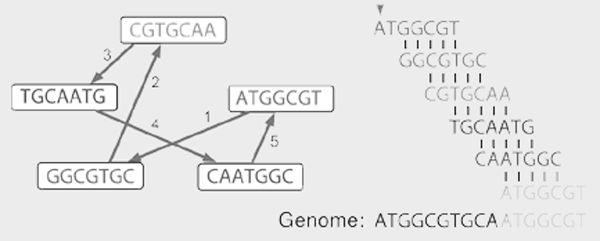
\includegraphics[width=0.66\textwidth]{figures/Introduction/thesis_2}
	\caption{\label{fig:assembly}\textbf{Assembly of Sanger sequences}\\
			(from \cite{compeau2011apply})}
\end{figure}

\subsubsection*{Annotation (I): gene calling}
Once that sequences with satisfactory length are obtained, the position of the ORFs (and other regulatory features) has to be extracted from the plain sequence: this process is known either with the term \textit{annotation} or \textit{gene calling}. Since experimental approaches are not affordable in term of time and cost, predictions have to be made to annotate the obtained sequence, taking advantage of the mechanisms of transcription and traduction and sets of experimentally validated gene annotations. The start codons are known to be ATG, GTG and TTG (especially in bacteria): given a random nucleotide sequence, we expect to find a stop codon every 60bp (5\% probability); however, it is known from the experiments that the average bacterial gene length is around 300bp. A first naive method would be then to find all the ORFs with length over 60bp: which indeed is the first step in many gene-calling softwares (see for instance prodigal \cite{hyatt2010prodigal}); however, the assumption that a genomic sequence has a random distribution is off course false, since each bacterial genomes has a distinct GC content, a distinct codon usage \cite{ermolaeva2001synonymous}, different intergenic regions sizes and the presence of signal sequences like the RBS: each bacterial species will therefore have a distinct gene signature. Gene calling algorithms take into account this species specific bias by using statistical models (like HMMs) and dynamic programming approaches, together classified under the name of \textit{ab initio} methods \cite{do2006computational}. 

\subsubsection*{Annotation (II): function assignement}
\begin{figure}[!tb]
	\center
    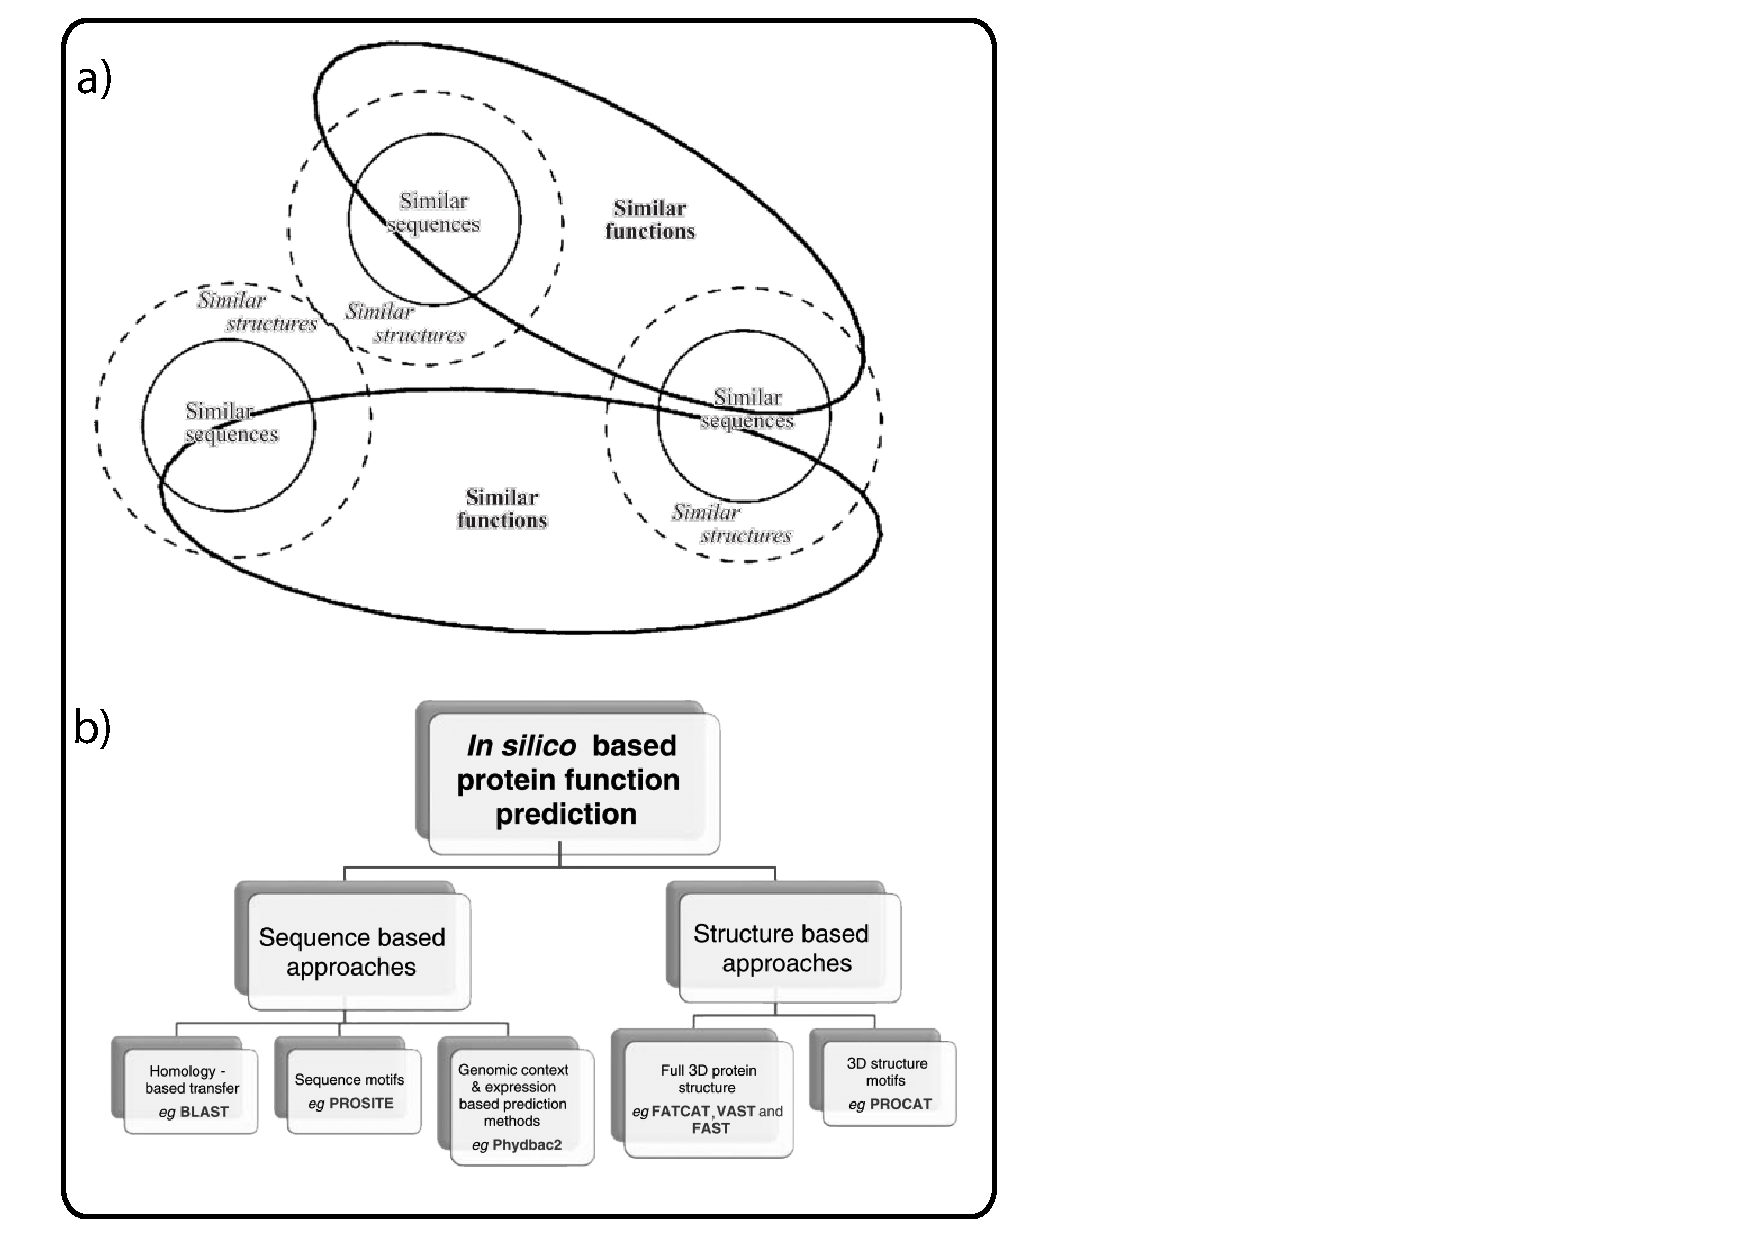
\includegraphics[width=0.66\textwidth]{figures/Introduction/thesis_3}
	\caption{\label{fig:funcannotation}\textbf{Functional annotation}\\
			a) Different patterns of functional similarity (from \cite{whisstock2003prediction}) \\
			b) Overview of functional annotation techniques (from \cite{sleator2010overview})}
\end{figure}

Given the high number of proteins that are annotated in each bacterial genome, experimental strategies to depict the function of each gene are not affordable; bioinformatic analyses are used instead, lead by the principle that proteins that exhibit a certain degree of similarity are probably evolutionary related and therefore should share similar functional features. This similarity can be measured at different levels: at the sequence level (through a BLAST \cite{camacho2009blast+} search on public databases) or at the structural level, which in some cases may be equivalent (Figure \ref{fig:funcannotation}a); the major problems in this transfer of function through homology is that there are no defined thresholds for this similarity measures and, most importantly, even closely similar sequences may exhibit very different functions. An important conseguence of this incorrect annotations is that the errors are propagated through each new sequenced genome in which a protein with enough similarity to the wrongly annotated protein is found \cite{whisstock2003prediction} \cite{sleator2010overview}. To overcome this problems, a series of alternative strategies have been developed: the use of curated protein databases (such as KEGG \cite{ogata1999kegg}) ensure a reduction of annotation errors and allows a partial metabolism reconstruction; the research of sequence motifs and domains instead of using the whole sequence allows a more granular and precise functional reconstruction, focusing on functional modules, which are less prone to ambiguations (see for instance INTERPRO \cite{apweiler2001interpro}\cite{zdobnov2001interproscan}) and, especially for bacterial genomes, the information about genomic context can be used to infer the function of a protein based on the known operons and genomic islands \cite{sleator2010overview} (Figure \ref{fig:funcannotation}b). All these automatic annotation methods are often refined by careful manual curators (i.e. as in the UNIPROT database \cite{uniprot2008universal}), which often take advantage of functional ontologies like GO \cite{ashburner2000gene} and experiments from the literature to better refine and correct the automatic annotations.

%HERE EXPAND WITH MORE DETAILS ON THE VARIOUS ANNOTATION TECHNIQUES?

\subsection{Bacterial genomics}
\label{sec:genemining}
Compared to partial sequences, complete (or even draft) genomic sequences allowed a wider array of analysis on a particular species: in fact, since all the functional repertoire of an organism is encoded in the genome, a complete reconstruction of the functions of an organism was theoretically possible, thanks to the functional annotation techniques described above; various analyses that were previously impossible have been made available thanks to bacterial genomics.

The presence of single genes or functions of interest could be easily tested looking for an homolog of an evolutionary related gene with known sequence; however, similar biological functions can belong to two proteins even if there is no evolutionary relationship (a phenomenon known as \textit{convergent evolution}), so the presence of a particular function must be checked by taking into account other sources of information, like the presence of a reaction in the metabolic network reconstruction (i.e. through KEGG), or the presence of a certain protein domain or the combination of two or more domains (i.e. through INTERPRO) in a gene, with the methods described above. This \textit{in-silico} approaches are often been referred as \textit{gene-mining} \cite{li2004gene}\cite{du2008functional}, which could help to reduce the amount of experiments needed to test the phenotype of an organism and the presence of a particular gene.

The potentials of bacterial genomics, however, are not limited to the analysis of a single gene or function, but indeed have been expanded to allow a broader and more general functional description of a bacterial species. One of the most powerful method that has been developed is based on the utilization of a controlled vocabulary (also termed as \textit{ontology}) of gene functions, divided in three macro-categories and with a hierarchical structure, with an increasing level of detail (Figure \ref{fig:gocog}a); this annotation categorization method is called the Gene Ontology \cite{ashburner2000gene}, and even if it was developed for eukaryotic species, it can also be applied to the bacterial kingdom. The three macro-categories were designed to address all the functional aspects of a gene product:

\begin{itemize}
\item \textbf{Biological process} is used to describe the biological objective of a gene: examples may be GO:0048591 (cellular growth) or GO:0009758 (carbohydrate utilization),
\item \textbf{Molecular function} describes the 	biochemical activity of a gene, including physical interactions: examples may be GO:0016874 (ligase activity) and GO:0003989 (acetyl-CoA carboxylase activity),
\item \textbf{Cellular component} describes where the function of the gene is expressed, a description that is more variable for eukaryotes than in bacteria: examples may be GO:0016020 (membrane) and GO:0043190 (ATP-binding cassette (ABC) transporter complex).
\end{itemize}

\begin{figure}[!tb]
	\center
    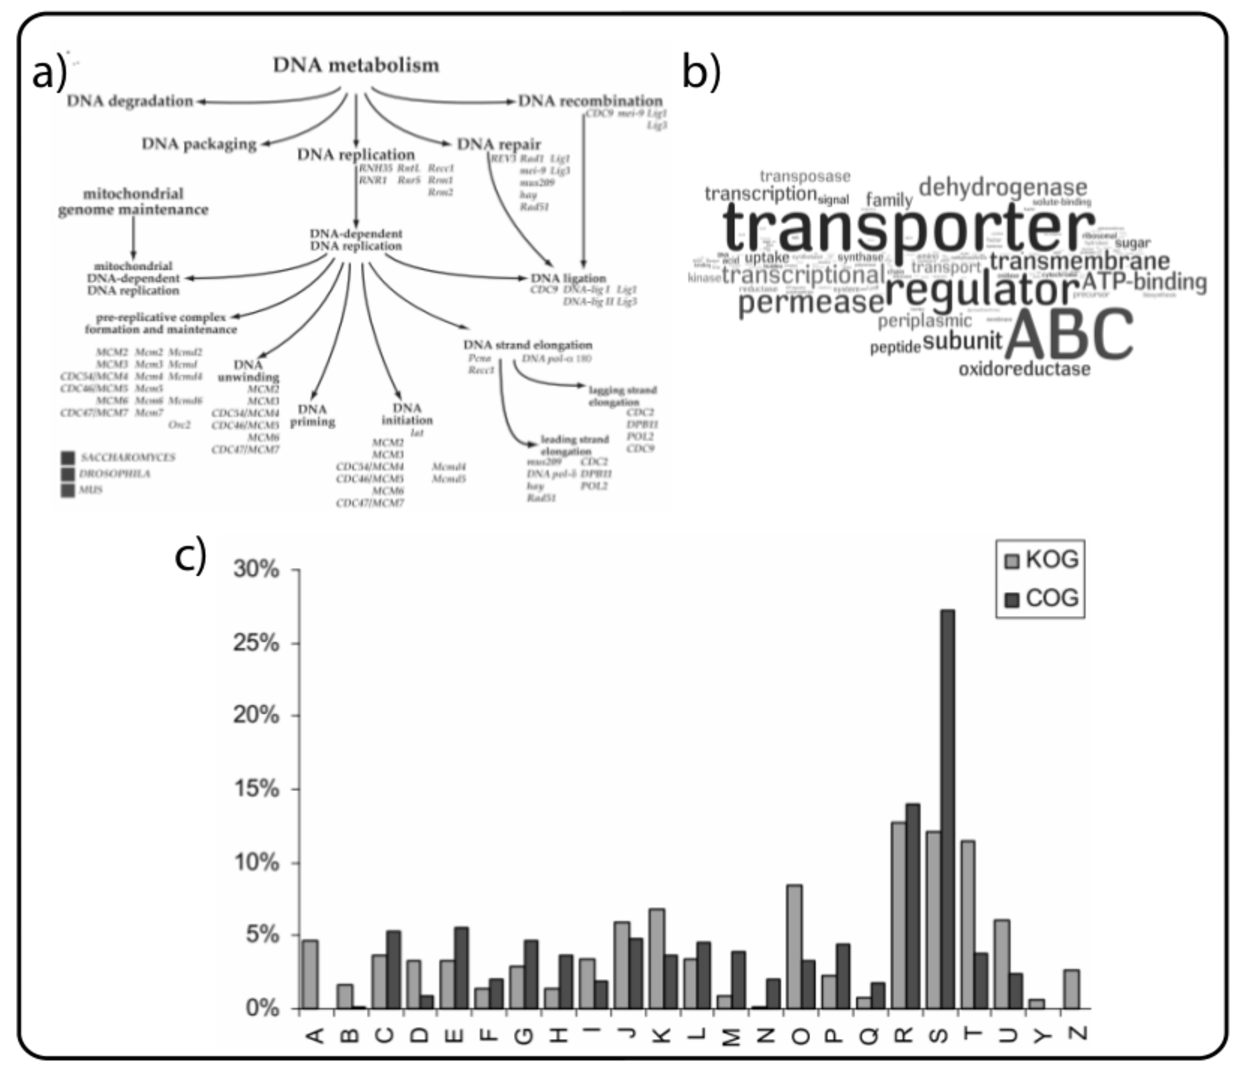
\includegraphics[width=0.77\textwidth]{figures/Introduction/thesis_4}
	\caption{\label{fig:gocog}\textbf{Functional categories}\\
			a) Example of the hierarchical structure of a GO annotation (from \cite{ashburner2000gene}) \\
			b) Word cloud of all the annotation terms found in \textit{S. meliloti} Rm1021; the size of each word is proportional to the frequency of the term (from \cite{wordcloud}) \\
			c) Broad functional categorization of prokaryotes (COG) and eukaryotes (KOG) (from \cite{tatusov2003cog})}
\end{figure}

The hierarchical structure of the gene ontology, with increasing levels of details allowed a precise and granular functional categorization of gene products, given the amount of experimental and predicted information available; most importantly, the ontologies can be updated with the results of new experiments and other evidences. Since all the proteins from a genome can be annotated using this method, an important consequence is that it is possible to construct an overall functional categorization of a given species (Figure \ref{fig:gocog}b), with the possibility to obtain a first general functional categorization of a species, which can be later compared to other organisms. The same approach can be applied using another annotation method with a general functional categorization, called COG \cite{tatusov1997genomic}\cite{tatusov2003cog}, which is a set of orthologs from all the three kingdoms of life (the current version has been built upon 66 genomes \cite{cogcategs}), each one belonging to one of the 25 macro-categories, further divided into single orthologs with a more precise functional categorization. Each protein can be assigned to a COG using rps-blast (reverse position specific blast) \cite{a1999impala}\cite{marchler2002cdd}, which allows to query a sequence against a library of position-specific scoring matrices (PSSMs) derived from each COG, thus assigning each protein to one (or more) COG categories; it is therefore possible to obtain a functional insight of the whole genome (with a lower degree of complexity, compared with GO), which again can be compared to other organisms (Figure \ref{fig:gocog}c).

\newpage
\section{From genomics to comparative genomics}
Describing the bacterial genomics as a series of analysis on a single organisms is indeed a rather big simplification: in fact, from the very beginning of the bacterial genomics era, questions regarding the genomic evolution were posed; the term \textit{comparative genomics} appeared then as soon as two bacterial genomes were available \cite{koonin1996complete}. Given that all life forms may have evolved from a last universal common ancestor (LUCA \cite{delaye2005last}\cite{koonin2005origin}), it is obvious to assume that many genes may be shared in all the three kingdoms of life, and in particular in the bacterial kingdom; the main goal is to understand which fraction of the genome is evolutionary conserved, which genetic traits have evolved through convergent evolution, and which genetic elements are specific to a particular taxa or to a single species. One of the most interesting questions that can be addressed through evolutionary comparative genomics is the analysis of the so-called \textit{minimal genome}, which theoretically is the minimum gene set able to support life; such a gene set should be present in all life forms, with genes involved in the replication of the genetic material, cell division and the core metabolism. Evidences of the presence of the minimal genome has been found already at the beginning of the genomics era, and more recent works have refined its putative size and gene content to about 200 genes \cite{koonin1996complete}\cite{koonin1996sequencing}\cite{gibson2008complete}.

%Comparative genomics is off course not only limited to evolutionary studies, but as soon as more genomes were available, was expanded to include other functional approaches (EXPAND OR REMOVE)

\subsection{Transferring functions: homologs, orthologs and paralogs}
The core foundation of comparative genomics analyses is the definition of the list of orthologs between two or more species: this term has seen many definitions during the recent history of biological science, which change significantly its biological meaning and the methods for its assesment \cite{altenhoff2009phylogenetic}. The first definition was given by Fitch in 1970 \cite{fitch1970distinguishing}, indicating those genes that have diverged through a speciation event; another, more practical definition of orthology is about function, as two orthologs are considered to exhibit the same function. The functional definition of orthology has an important consequence: annotations can be transferred from one genome to another when the orthologs are defined, thus avoiding the need for experimental validations of functions; most importantly, two genomes can be easily compared to highlight functional differences. However, since the lack for an univocal definition of protein function, this approach has to be taken with caution to avoid propagations of incorrect annotations, as well as a series of directed experiments to validate the transferred functional annotation. Another important feature of orthologous relationships is that the orthology information is not transitive, meaning that if a third protein has to be added to an existing pair of orthologs, each pairwise analysis has to be conducted separately \cite{altenhoff2009phylogenetic}.

%USE OF ORTHOLOGS IN C:GENOMICS?
\subsubsection{Orthologs and paralogs}
\begin{figure}[!tb]
	\center
    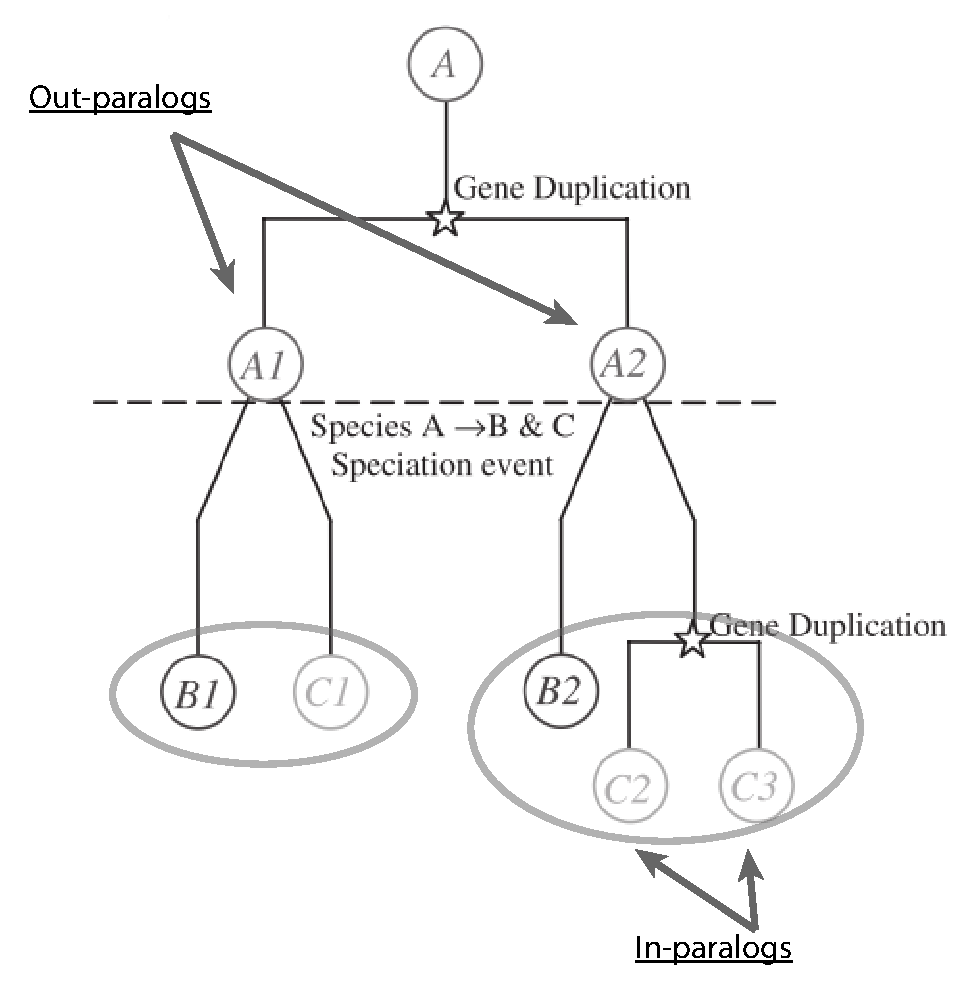
\includegraphics[width=0.77\textwidth]{figures/Introduction/thesis_5}
	\caption{\label{fig:orthologs}\textbf{Orthologs and paralogs}\\
			Distinction between out-paralogs and in-paralogs; grey elipses indicate orthologs (modified from \cite{o2005inparanoid})}
\end{figure}
Since the evolution of bacterial genomes doesn't rely only on mutations at the single nucleotide level, but instead consists also of recombinations, deletions and duplications, an additional category of orthologs (\textit{paralogs}) has to be considered to include gene duplication events: they are, in theory \textit{bona-fide} orthologs as the original copy. An important distinction however has to be made, since several examples in eukaryotes have shown that some paralogs have diverged so much from the original copy to the point were the function is significantly altered \cite{studer2009confident}\cite{nehrt2011testing}; the proposed distinction is between \textit{out}-paralogs, whose duplication events occurred before the speciation event, and \textit{in}-paralogs, whose duplication occurred after the speciation event \cite{remm2001automatic} (Figure \ref{fig:orthologs}). Out-paralogs, although retaining a significant degree of homology and a putative similar function, are not to be considered orthologs, while the in-paralogs are most likely to retain the same function.

\subsubsection{Algorithms to infer orthology}
Many algorithms have been developed for the assessment of orthology, and many of them have been scaled up to allow the analysis on whole genomic sequences: they can be roughly divided in two main categories, according to the main source of information for the orthology calling (Table \ref{tab:orthologs}).

\begin{table}
    \begin{tabularx}{\textwidth}{|p{2.9cm}|p{5.3cm}|p{3.6cm}|}
        \hline
        \textbf{Method} & \textbf{Features} & \textbf{Examples} \\ \hline
        Tree based & Construction of phylogenetic trees, followed by reconciliation with species tree & Ensembl compara \cite{kersey2010ensembl}, LOFT \cite{van2007orthology}, TreeFam \cite{li2006treefam} \\ 
        Homology based & Sequence similarity measures, followed by clusterization techniques & BBH, COG/KOG \cite{tatusov1997genomic}\cite{tatusov2003cog}, InParanoid \cite{o2005inparanoid} \& Multiparanoid \cite{alexeyenko2006automatic}, OrthoMCL \cite{li2003orthomcl}, EggNOG \cite{jensen2008eggnog} \\ 
        Other & Pairwise evolutionary distances, reciprocal smaller distances, gene context conservation & RoundUp \cite{deluca2006roundup}, Homologene \cite{wheeler2007database}, OMA \cite{dessimoz2005oma} \\
        \hline
    \end{tabularx}
	\caption{\label{tab:orthologs}\textbf{Overview of orthology assesment methods}}
\end{table}

\paragraph{Tree based}
The first method to be implemented was based on the construction of a multiple sequence alignment tree and its comparison with the analyzed species tree to infer the orthologs clusters, a method called \textit{reconciliation}. Although this method has proven to be precise, it's extremely time consuming, since it usually requires a manual curation step to resolve the tree conflicts, so it's usually used for small gene families; moreover, horizontal gene transfer events (HGT) may alter the sequence tree topology, rendering this method particularly tricky for bacterial genomes, where HGT is very common.

\paragraph{Homology based}
The presence of complete bacterial genomes has led to the development of new automatic methods for orthology assesment, which allow the analysis of whole bacterial genomes in a reasonable amount of time; these methods are based on homology measures (since orthologs are also homologs, even though the contrary is not necessarily true \cite{altenhoff2009phylogenetic}), which lead to the definition of an homology matrix between each protein pair that has then to be clusterized to extract the orthologs. These methods are characterized by an higher number of false positives, because of events such as gene losses, but can work even for big phylogenetic distances. Most of the algorithms based on this method use Blast for the homology measure, with different clusterization methods. The most simple implementation of this method is the so-called Bidirectional Best Hit (BBH, Figure \ref{fig:bbh}): the orthologs of genome A are defined as those proteins whose best match in genome B have the same protein as best match in genome A. All the other algorithms rely on this concept, while changing the various filters and clusterization steps: InParanoid for instance allows the definition of paralogs, which cannot automatically be defined by naive BBH algorithms.

\begin{figure}[!tb]
	\center
    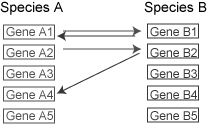
\includegraphics[width=0.5\textwidth]{figures/Introduction/thesis_6}
	\caption{\label{fig:bbh}\textbf{BBH algorithm}\\
			Schematic function of the BBH algorithm: the first two proteins are orthologs, the other three are just homologs (from \cite{bbh})}
\end{figure}

\subsection{The revolution in sequencing technologies}
\label{sec:revolution}
The last decade has seen a series of impressive developments in automatic sequencing technologies, with the creation of many new techniques and platforms: compared to the first era of genomes sequencing, biologists now can decide which technology is best suited for their analysis. All these new developments have been termed \textit{Next-generation Sequencing} (NGS), including also the latest automatic Sanger sequencing technologies \cite{glenn2011field}; even though there are many platforms available, the NGS technologies are usually divided in three distinct generations, according to their peculiarities:

\begin{itemize}
\item \textbf{1\textsuperscript{st} generation:} capillary Sanger sequencing through dye-terminator,
\item \textbf{2\textsuperscript{nd} generation:} platforms that require amplification of the template sequence prior to the sequencing step,
\item \textbf{3\textsuperscript{rd} generation:} platforms that directly sequence individual DNA molecules.
\end{itemize}

Even if the first reports about the NGS techniques are dated in 1996 \cite{ronaghi1996real}, the first commercial applications of the pyrosequencing technologies appeared in 2005; since then, each year has seen the development of new instruments and variations, with a considerable drop in the cost/Mb. The major platforms used today are listed below (Table \ref{tab:ngs}, Figure \ref{fig:ngs}).

\begin{table}
    \begin{tabularx}{\textwidth}{|p{2cm}|p{5.3cm}|p{2.8cm}|p{1.2cm}|}
        \hline
        Platform    & Sequencing method          & Amplification method & Reads-length \\ \hline
        454         & Synthesis (pyrosequencing) & emPCR                & 400-700      \\ 
        Illumina    & Synthesis                  & BridgePCR            & 100          \\ 
        SOLiD       & Ligation                   & emPCR                & 35-75        \\ 
        HeliScope   & Synthesis                  & ~                    & 35           \\ 
        Ion Torrent & Synthesis (H\textsuperscript{+} detection)   & emPCR                & 100         \\ 
        PacBio      & Synthesis                  & ~                    & 860-1100     \\
        \hline
    \end{tabularx}
    \caption{\label{tab:ngs}\textbf{Overview on NGS sequencing platforms} (adapted from \cite{glenn2011field})}
\end{table}

\paragraph{454} The first NGS technology to be implemented, in which single template molecules are amplified through \textit{emPCR} (emulsion PCR), a technique in which each DNA molecule is trapped inside aqueous droplets together with a primer-coated bead and the PCR reagents; later each bead is trapped inside a picotitre plate designed to contain exactly one bead for well. The sequence is then read through pyrosequencing: a dNTP is added on the plate, together with the enzymes DNA polymerase, ATP sulfurylase, luciferase and apyrase, and with the substrates adenosine 5'  phosphosulfate (APS) and luciferin; the incorporation of a dNTP releases pyrophosphate, which is converted, together with adenosine 5' phosphosulfate, into ATP by the enzyme ATP sulfurylase: the ATP is then used by the luciferase to convert luciferin to oxyluciferin that generates light. The amount of light emitted by each well is directly proportional to the number of bases that were incorporated by the DNA polymerase.

\paragraph{Illumina} Formerly known as Solexa, this technology is based on the adhesion of the template sequences to a special glass surface with a series of single-strand primers complementary to the adaptors ligated to the templates; the single templates are amplified through \textit{Bridge PCR}, obtaining a series of clusters containing many copies of the same template. Sequencing is achieved through the contemporary addiction of four dNTPs labelled with fluorescent dyes, which are read with a camera. Compared with 454, Illumina reads are usually shorter, but with an higher sequencing depth.

\paragraph{SOLiD} Unlike the previous platforms, the SOLiD technology obtains the sequences through ligation, instead of synthesis; the template preparation is similar to 454, with emPCR apmlification on beads, ligated to a glass surface. The actual sequencing step involves the utilization of all the possible di-NTPs, each one labeled with a different fluorescent dye; many different cycles involving different primers are used, leading to a double reading of each base. This technology yields reads that are significantly shorter than the others, but with an higher accuracy and depth.

\paragraph{HeliScope} The first single-molecule sequencing platform to be developed, performs sequencing through the addiction of each fluorescently labeled dNTP and the subsequent read through a laser camera. Read sizes are comparable to the SOLiD platform.

\begin{figure}[!htb]
	\center
    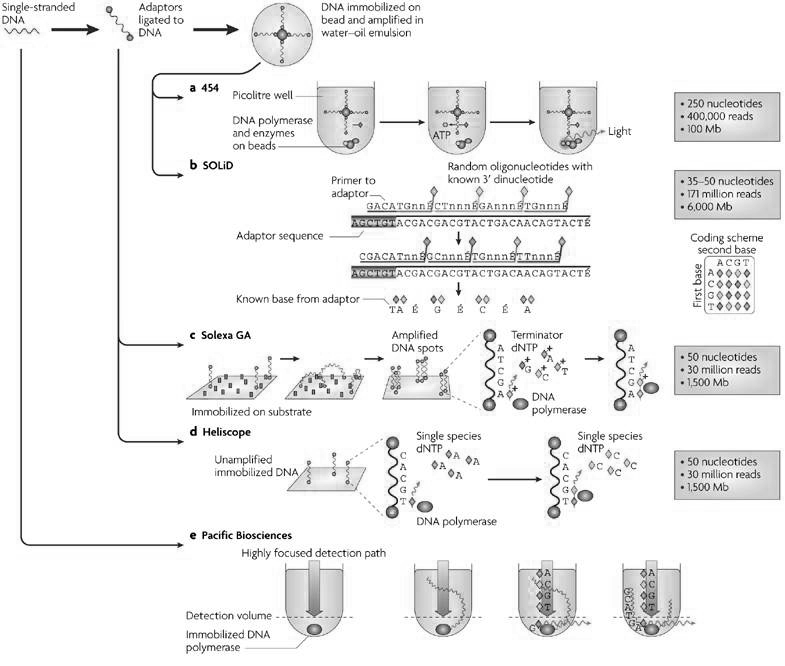
\includegraphics[width=1\textwidth]{figures/Introduction/thesis_7}
	\caption{\label{fig:ngs}\textbf{NGS overview}\\
			Main features of the NGS technologies, except the Ion Torrent platform (from \cite{maclean2009application})}
\end{figure}

\paragraph{Ion Torrent} This platform has the distinctive feature, compared the the others: it doesn't need a camera for the recognition of the incorporated dNTPs, thus reducing the size of the corresponding apparatus and increasing the speed of the analysis. In this technique, each DNA molecule is incorporated in a well inside a semiconductor chip, together with the enzyme DNA polymerase: the dNTPs are added sequentially, with the release of a proton when the nucleotide is incorporated, which is detected by an ion sensor. The amount of electronic signal is directly proportional to the number of dNTPs that have been added to the growing strand (Figure \ref{fig:ion}). 

\begin{figure}[!b]
	\center
    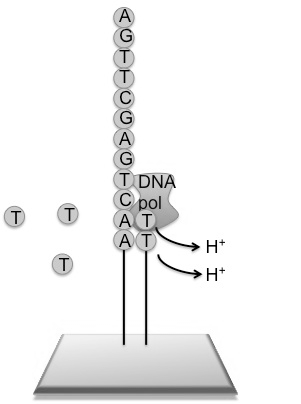
\includegraphics[width=0.33\textwidth]{figures/Introduction/thesis_8}
	\caption{\label{fig:ion}\textbf{Ion Torrent technology}\\
			Schematic function of the Ion Torrent sequencing by synthesis with proton detection (from \cite{ion})}
\end{figure}

\paragraph{PacBio} This technology is also known as single molecule real time sequencing, in which single DNA molecules are present inside microscopic wells, with a molecule of the enzyme DNA polymerase at the bottom; each fluorescent dNTP is added sequentially, and its incorporation is detected through a camera: a single nucleotide incorporation can be detected, thanks to the use of zero-mode waveguide wells, which confer particular properties to light \cite{eid2009real}. Compared to the other NGS sequencing technologies, this platform allows reads with mean length of about 1000bp, comparable to Sanger sequencing.

\begin{figure}[!htb]
	\center
    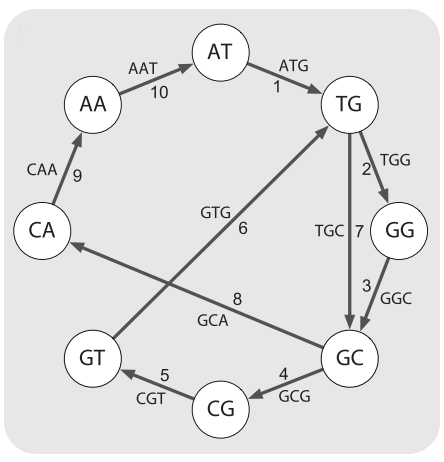
\includegraphics[width=0.7\textwidth]{figures/Introduction/thesis_9}
	\caption{\label{fig:debrujin}\textbf{Assembly through de Brujin graphs}\\
			Schematic representation of a de Brujin graph with k-size 3 (from \cite{compeau2011apply})}
\end{figure}

Compared to tradional Sanger sequencing (section \ref{sec:hamiltonian}), the amount of sequences produced by the NGS technologies (especially for Illumina), poses serious problems for genome assembly through hamiltonian cycles algorithm, whose efficiency is strongly reduced also by the relatively low average length of the reads, with the need to perform a really high number of alignments (in fact, this algorithm is \textit{NP-complete}, meaning that an optimal solution for this problem may not exists). These limitations have been addressed in NGS sequences assembly with the adoption of the so-called \textit{de Brujin} graphs \cite{compeau2011apply}: the graph is constructed with the adoption of sequences \textit{k-mers} (with k values usually below half of the average read length). Each node of the graph is composed by all the k-1 mers that are found in the reads pool, with an edge between two nodes if exists a k-mer that has two nodes as prefix and suffix (Figure \ref{fig:debrujin}); the assembly is then obtained through an eulerian cycle search, that is a cycle in which each edge is visited exactly once, an algorithm approach with reduced complexity. The same problems as hamiltonian algorithms are off course still present, like the presence of duplicated sequences, but many assemblers have already been developed to solve these problems \cite{simpson2009abyss}\cite{boisvert2010ray}\cite{zerbino2008velvet}. 

\subsection{One species, many sequences}
\begin{figure}[!tb]
	\center
    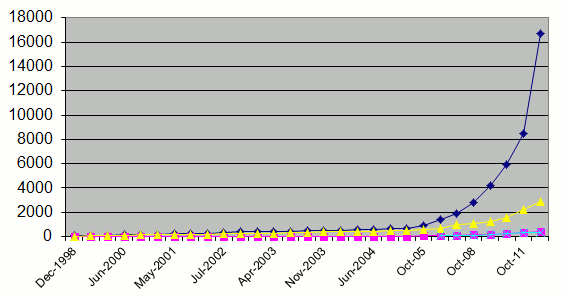
\includegraphics[width=1\textwidth]{figures/Introduction/thesis_10}
	\caption{\label{fig:gold}\textbf{Genome projects according to phylogenetic group }\\
			Number of genome projects registered in the GOLD database, October 2012 (from \cite{gold}). Blu line, bacteria; pink line, archea; yellow line, eukarya; cyan line, mammals.}
\end{figure}

The proliferation of such an high number of new sequencing technologies, each one in competition with the others, has lead to a dramatic drop in the complete genomic sequencing costs, leading to the definition of new terms and of the comparative genomics analysis. The first tangible conseguence is the higher number of genomic sequences that are added to public databases each year, with a prominent role of bacterial species, which outnumber any other taxonomical group (Figure \ref{fig:gold}); in fact the number of available bacterial genomic sequences in the NCBI repository are 2171 (on November 2012), with many more sequences available each day, as all the genome projects are closed and the data submitted. Not all these new projects and sequences belong to distinct species, but in many cases many genomes for each species are available (Figure \ref{fig:intraspecies}). The term comparative genomics was then expanded to include those analysis between genomes coming from the same species, with important functional and evolutionary applications.

\begin{figure}[!tb]
	\center
    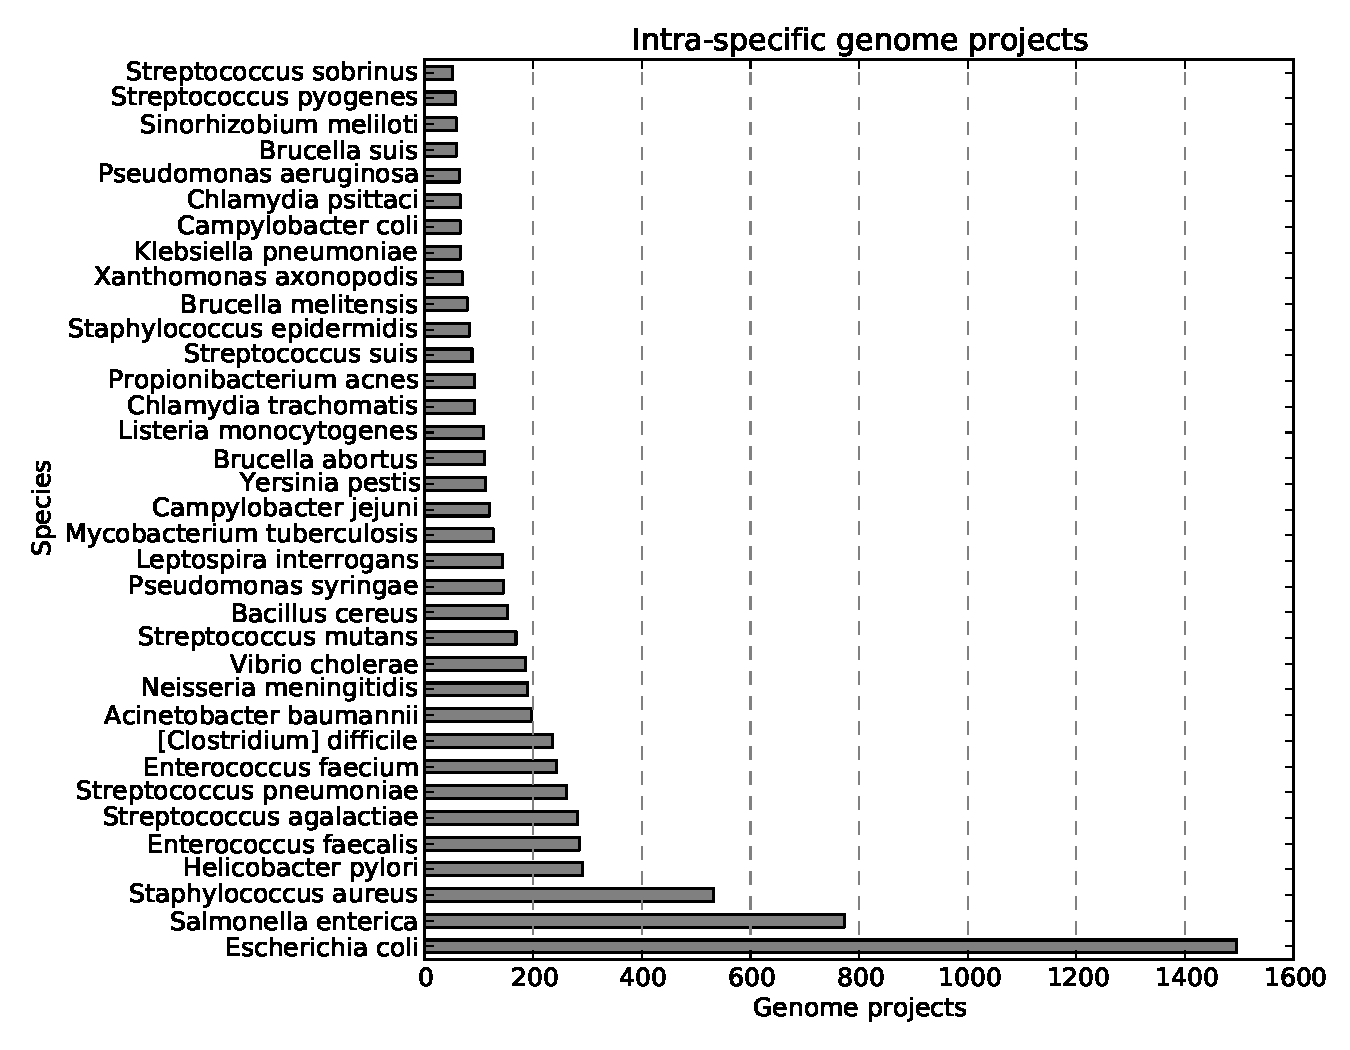
\includegraphics[width=1\textwidth]{figures/Introduction/thesis_11}
	\caption{\label{fig:intraspecies}\textbf{Bacterial species with more than 50 genomic projects}\\
			Number of genome projects registered in the GOLD database, October 2012 (from \cite{gold}).}
\end{figure}

\subsection{Intra-specific comparative genomics}
The species concept is challenged by the bacterial world, since a morphological and functional categorization of a bacterial species is not defined and certain, and also genetically, the low barriers on genetic exchange between bacteria (HGT events, transduction, transformation, ecc.) poses serious doubts on the application of the species label to a bacterial entity, even though markers such as the 16s rRNA can still be used. Given the high functional variability inside a so-called bacterial \textit{species}, interesting questions have been posed on which fractions are conserved and which ones are variable inside a genome and how it evolves inside a species. The strategies to address these question involve the genome comparison, through the definition of all the orthologous groups inside a genome, in order to highlight those genes that are common to all the analyzed strains and those that are specific to one or more strains: the whole orthologous groups set inside a set of genomes has been termed \textit{pan-genome}, after the observation that new genes are always discovered when a new genome of a particular species is sequenced \cite{tettelin2005genome}\cite{medini2005microbial}. The pangenome could be therefore used to describe the overall functional repertoire of a species, and most importantly to define the dynamics of acquisition and loss of such functions.

\subsubsection{Core, accessory and unique genome}
The orthologous groups that are part of a microbial pangenome can be further divided in other catogories, according to their occurrence in the analyzed strains:

\begin{itemize}
\item \textbf{Core genome:} orthologs that are present in each genome,
\item \textbf{Dispensable genome:} orthologs that are present in one or more genomes, but not in all,
	\begin{itemize}
		\item \textbf{Accessory genome:} orthologs that are present in two or more genomes, but not in all,
		\item \textbf{Unique genome:} orthologs that are present only in one genome.
	\end{itemize}
\end{itemize}

The core genome, which in some bacterial species can account for nearly half of the pangenome (and with a significant fraction exhibiting identical sequences also at the nucleotide level), is thought to contain house-keeping functions and those genes that define the core metabolism and phenotype of the species; the dispensable genome instead is thought to harbor functions related to environmental adaptation and survival in strain-specific echological niches, with the unique genome more specific to the functions of a single strain \cite{medini2005microbial}. Moreover, a particular kind of unique orthologs are the so-called \textit{ORFan} genes, that are those genes that have no significant similarity to any gene previously sequenced and present in public databases, whose origin can be probably tracked down to mutations of intergenic regions, which are then targeted by random mutations and selection, before being fixed in the genome \cite{yomtovian2010composition}. Given the presence of such "new" genes with low or none homology to known proteins, the dispensable fraction contains more genes with unknown or poor functional categorization, which poses serious problems in the functional categorization of a species pangenome. On the other hand, comparative genomics can help in the correction of annotation errors, and especially in the case of incorrect gene predictions, thanks to the presence of core orthologs: in fact, some programs that allow the correction of gene annotations have already been developed \cite{samuel12improving} (Figure \ref{fig:mugsy}).
The most important application of intra-specific comparative genomics for the scope of this thesis is the possibility to explain the phenotypic variability through the pangenome analysis, and in particular the fraction of the phenotypic variability that can be explained by the presence/absence pattern of one or more genes, an information that is all included in the pangenome. Through this approach, a series of possible gene candidates for the loss/gain of function in a particular strain can be highlighted and proposed for confirmation experiments: the gene mining approach previously described (section \ref{sec:genemining}) should be then applied to the dispensable genome fraction, with an analysis on the available annotations, grouped by orthologs.

\begin{figure}[!tb]
	\center
    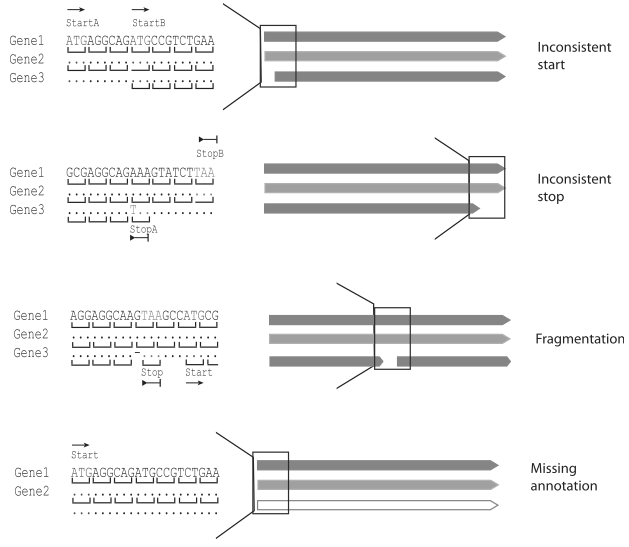
\includegraphics[width=0.66\textwidth]{figures/Introduction/thesis_12}
	\caption{\label{fig:mugsy}\textbf{Incorrect gene annotations}\\
			 Examples of incorrect gene calling that can be corrected thanks to comparative genomics (from \cite{samuel12improving})}
\end{figure}

\subsubsection{Open and closed pangenomes}
\begin{figure}[!tb]
	\center
    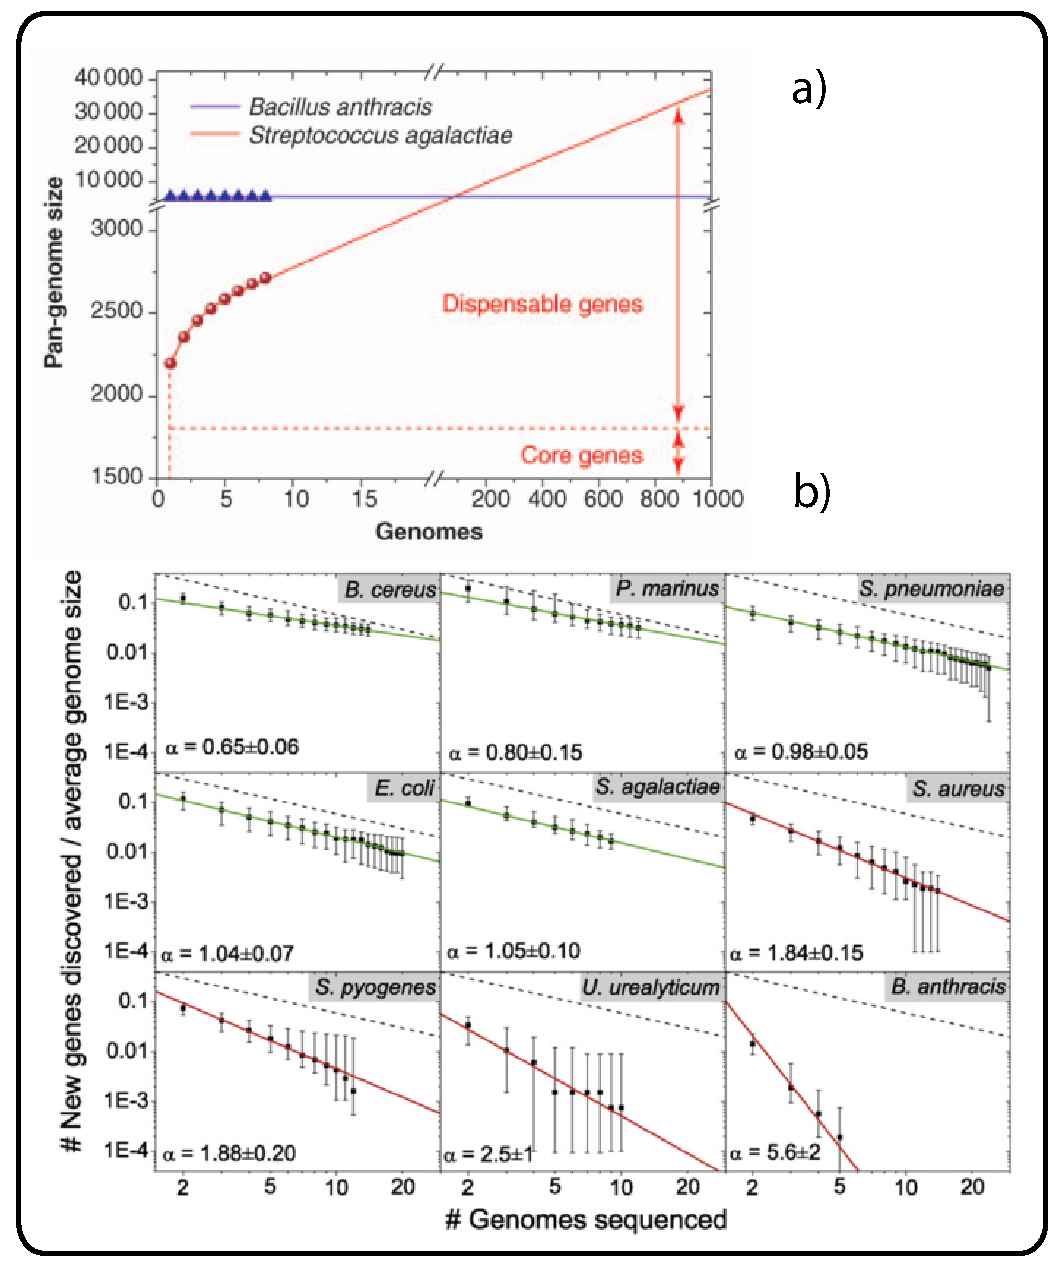
\includegraphics[width=0.8\textwidth]{figures/Introduction/thesis_13}
	\caption{\label{fig:openclosed}\textbf{Open and closed pangenomes}\\
			a) Comparison of the pangenome rarefaction curve between open (\textit{S. agalactiae}) and closed (\textit{B. anthracis}) pangenomes (from \cite{medini2005microbial})\\
			b) Comparison of the new genes discovery rate between open (red lines) and closed (green lines) pangenomes (from \cite{tettelin2008comparative})}
\end{figure}

Another interesting property of the bacterial pangenome is the possibility to infer the lifestyle and the genome evolution of a species solely on the basis of the pangenome rarefaction curve. When the term pangenome was defined, two distinct tendencies in pangenome dynamics were noted: for some genomes many new genes were found for each new genome added to the pangenome, while for some others a significantly smaller amount of new genes were added for each new genome \cite{medini2005microbial} (Figure \ref{fig:openclosed}a). The assumption is that genomes with an evergrowing pangenome probably belong to many and different environments, thus needing a larger gene set to be able to cope with the various nutrients and stress conditions; on the other hand, pangenomes with a relatively low rate of new genes for each genome are probably those that experience a low habitat variability and therefore exhibit a stable genome, like pathogens and obligate symbionts. This observation has been further refined with other genomes, leading to the classification in open and closed pangenomes, described by the fit to the Heaps' law (Equation \ref{eq:heap}): when the $\alpha$ parameter, defined by the fit of the heaps' law to the pangenome rarefaction curve, is $\leq$ 1 the pangenome is described as open, while with $\alpha >$ 1 the pangenome is described as closed. Indeed the species that are found to have a closed pangenomes belong to pathogens and obligate symbionts, like \textit{B. anthracis}, \textit{S. aureus} or \textit{B. aphidicola}, while free-living species like \textit{B. cereus}, \textit{E. coli} or \textit{S. meliloti} are found to have an open pangenome \cite{tettelin2008comparative} (Figure \ref{fig:openclosed}b).

\begin{equation}
\label{eq:heap}
n \sim N^{-\alpha}
\end{equation}

% Here genomic fluidity

\newpage
\section{A tale of two cities: plant-bacteria interaction}
\label{atale2cities}
The bacterial kingdom it's not important just on its own, but also when considering its impact on higher organisms, such as animals, plants and fungi; in recent years, the awareness on the importance of such interactions have grown, with many long-term projects being funded: a notable example is the human microbiome project, aimed at the understanding of the role of the bacterial communities inhabiting the human body in health and physiology \cite{turnbaugh2007human}.

The interaction that is more relevant for this thesis is the plant-bacteria interaction, which indeed is complex and involves a vast range of organisms, strategies and impacts on plants; most importantly, this interactions have been proven to have serious impacts on agriculture, in both economic and environmental terms. These bacteria are often grouped together under the definition of \textit{plant associated bacteria}, but there are many different kinds of plant-bacteria interactions, depending on the occupied niche and on the role in that this bacteria play in the interaction.

\textbf{Occupied plant niche}:
\begin{itemize}
\item \textbf{Endophytes:} those bacteria that colonize the internal tissue of the plant showing no external sign of infection or negative effect on their host \cite{holliday2001dictionary}\cite{schulz2006microbial}; they are further classified as obligate or facultative endophytes. Obligate endophytes are dependent on the plant for their growth and survival, thus being transmitted only through seeds or vectors, while facultative endophytes can also grow in other environments, like the rhizosphere \cite{ryan2007bacterial} (Figure \ref{fig:plantendophytes}).
\item \textbf{Rhizospheric bacteria:} those bacteria inhabiting the plant roots surface and the immediate surroundings where plant essudates are released and stimulate bacterial growth \cite{haas2005biological}; a soil region known as \textit{rhizosphere}, where bacteria play a role in providing nitrogen and phosphorous to the plant, in the protection from parasites and pathogens and in the maintenance of soil structure \cite{singh2004unravelling}.
\item \textbf{Phyllospheric bacteria:} those bacteria inhabiting the surfaces of the plant aerial tissues (also defined as \textit{above ground} tissues), especially on the leaves; these bacteria are also called \textit{epiphytes} \cite{lindow2003microbiology}, and they have a great influence on plant fitness and productivity \cite{whipps2008phyllosphere}.
\end{itemize}

\begin{figure}[!t]
	\center
    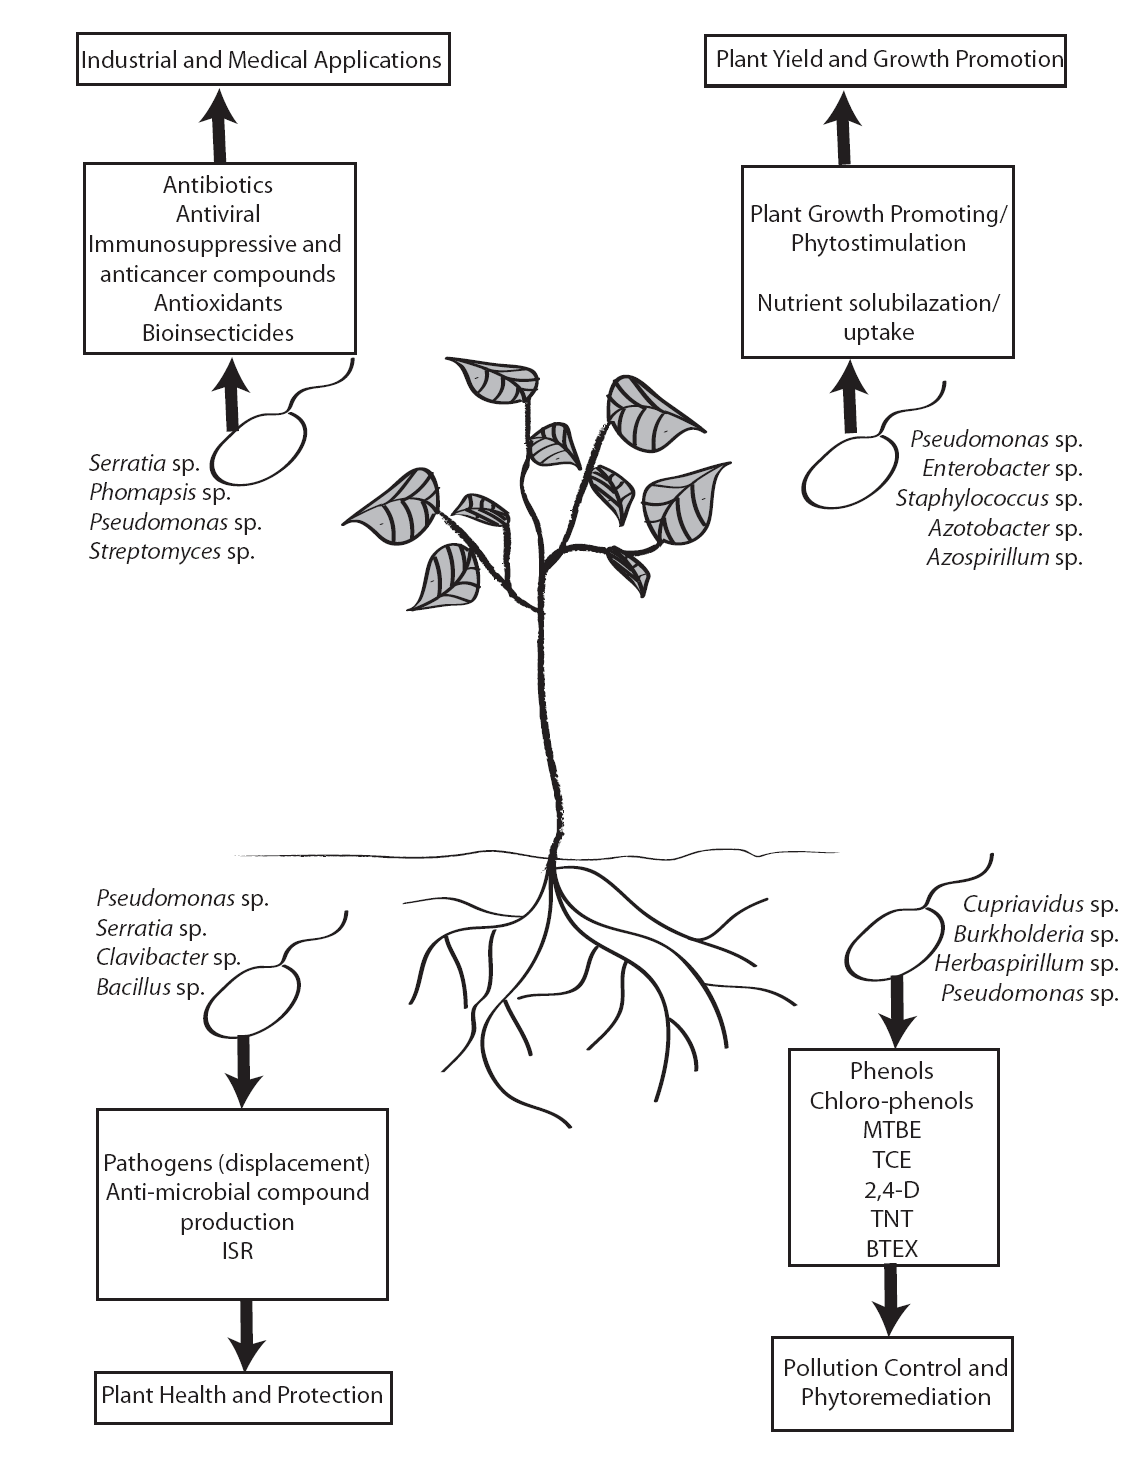
\includegraphics[width=0.7\textwidth]{figures/Introduction/thesis_14}
	\caption{\label{fig:plantendophytes}\textbf{Main players and effects of plant endophytes}\\
			The main species involved in the endophytic interaction and their effect on plant are reported (from \cite{mengoni2011bacterial}, adapted from \cite{ryan2007bacterial})}
\end{figure}

Some bacteria are indeed capable to occupy more than one of this niches, the most notable example being the facultative endophytes, which often inhabit the rhizosphere, later invading plant tissue from cracks in lateral roots or in roots elongation and differentiation zones, probably thanks to the production of cellulolytic and pectinolytic enzymes; the plant is then quickly colonized, with bacterial cells found in the aerial  tissues after one day \cite{rosenblueth2006bacterial}\cite{hallmann1997bacterial}.

All the bacteria that interact with plants can be additionally classified according to their role in the interaction: they can be either commensals, sharing and exchanging nutrients with the plant, pathogens, with deleterious effects on plant health, or symbionts, with a mutualistic interaction.

\begin{figure}[!t]
	\center
    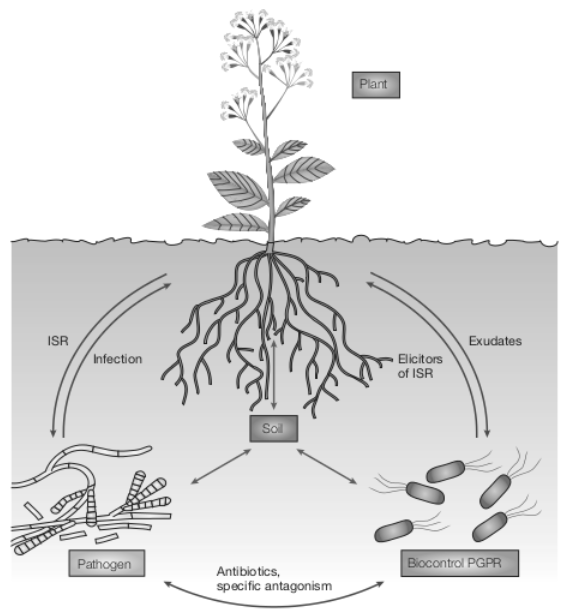
\includegraphics[width=0.7\textwidth]{figures/Introduction/thesis_15}
	\caption{\label{fig:plantprotection}\textbf{Interactions between biocontrol plant growth-promoting rhizobacteria, plants, pathogens and soil}\\
			From \cite{haas2005biological}}
\end{figure}

A particular class of rhizospheric bacteria interacting with plants are termed together under the name \textit{plant growth-promoting rhizobacteria} (PGPR), indicating those bacteria that have a positive impact on plant health and growth. Plant growth is promoted either by protection mechanisms than by nutrient supply: in fact, the  effects of PGPR on plants are divided in indirect and direct; indirect effects include antibiotic protection against pathogenic bacteria, reduction of iron available to phytopathogens in the rhizosphere and exclusion of pathogens by competition (Figure \ref{fig:plantprotection}), while direct effects include the provision of bioavailable phosphourus, nitrogen fixation, syderophore production for plant iron uptake, productions of plant hormonoes and the modulation of the induced systemic resistance (ISR) \cite{vessey2003plant}\cite{lucy2004applications}. This functions can be carried on either by endophytes or symbionts: in fact, some bacterial species can exhibit both plant association phenotypes, like the alphaproteobacterium \textit{Sinorhizobium meliloti} \cite{pini2012exploring}.

%All this beneficial effects take a considerable part in the natural and anthropic plant biology

\subsection{Symbiosis and biological nitrogen fixation}
One of the most important phenotypes that influences plant growth and that has a tremendous impact on agriculture it's the \textit{biological nitrogen fixation} (BNF) process; in fact nitrogen, as one of the most important chemical elements in life, is crucial for a successful plant growth. Nitrogen is an abundant chemical element mainly present as N\textsubscript{2} in the atmosphere (10\textsuperscript{15} tons), with 10\textsuperscript{9} tons that enter the nitrogen cycle each year \cite{postgate1982fundamentals}; the transformation of nitrogen into more available chemical forms has many known mechanisms, both biological and not, such as lightning (supplying 10\% of the annual fixed nitrogen \cite{sprent1990nitrogen}), BNF and anthropogenic chemical N\textsubscript{2}-fertilizers. Today 25\% of the total annual fixed nitrogen comes from anthropogenic chemical nitrogen fixation, while about 60\% comes directly from BNF \cite{peoples1995biological}; the use of N\textsubscript{2}-fertilizers however, has many drawbacks: is expensive, relies on fossile fuels, thus contributing to the climate change, and its usage leads to nitrate water contamination and other pollutions concerns. For this reasons, being able to control the BNF process is a key milestone towards a sustainable agriculture \cite{stewart1966nitrogen}, also considering the growing food safety concerns, especially in less developed countries \cite{n2africa}; on the economic side, the adoption of BNF as the main source of nitrogen for agricultural fertilization would greatly reduce the costs, since about 90 millions tons of nitrogen per year are made available through BNF. 

One of the most important sources of BNF is inside the leguminous plants roots, where rhizospheric bacteria establish a symbiotic interaction, providing fixed nitrogen to plants in exchange of nutrients; this interaction happens inside the plant roots, often in specialized organs called \textit{nodules}. Many bacterial species are able to perform BNF inside leguminous plants, belonging to the alpha and beta proteobacteria subclasses \cite{chen2003legume}. One of the most studies bacterial species associated with leguminous plants is the alphaproteobacterium \textit{Sinorhizobium meliloti}, which establishes a symbiotic relationship with the plant \textit{Medicago sativa} (also termed \textit{alfalfa}). Alfalfa is a perennial leguminous plant from the \textit{Fabaceae} family, known for its resistance to drought and extreme temperatures, but mainly for its high productivity, its nutrients content and its role in soil quality improvement; it's the most cultivated legume in the world, being used as forage, as crop for bioenergy and for the recovery of degraded or marginal lands \cite{vance2001application}\cite{ane2007recent}\cite{bouton1996new}\cite{comisalfalfa}; recently, also the biofuels industry has conducted pilot studies for the utilization of this plant as a source of energy, through the gasification process, using the resulting ashes as fertilizers \cite{mozaffari2000corn}\cite{mccaslin2007future}. The overall world alfalfa production was 436 million tons in 2006, with the United States as the lead producer and Argentina, Australia and South Africa as the other main producers \cite{alfalfa} (Figure \ref{fig:alfalfa}). Thanks to the symbiosis with rhizobial species, alfalfa has an important role in the management of agricoltural lands fertility, and in particular in keeping the bioavailable nitrogen available to other coltures, thus reducing land depletion and the use of chemical fertilizers.

\begin{figure}[!tb]
	\center
    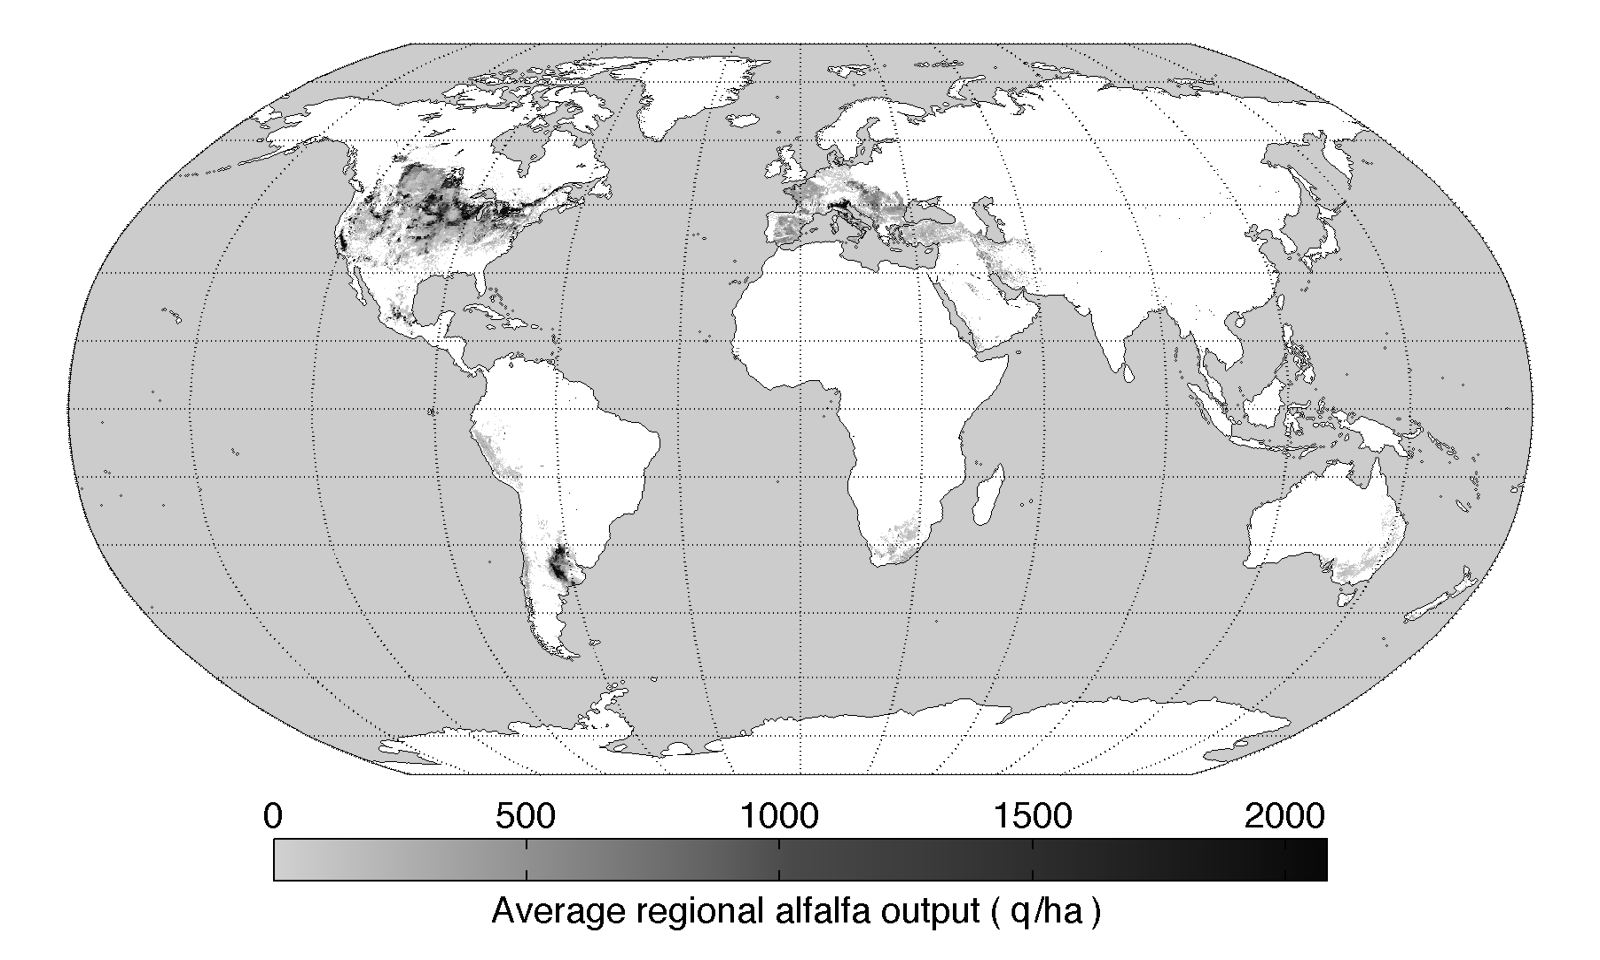
\includegraphics[width=1\textwidth]{figures/Introduction/thesis_16}
	\caption{\label{fig:alfalfa}\textbf{World alfalfa production}\\
			From \cite{alfalfa}}
\end{figure}

The symbiosis between \textit{M. sativa} and \textit{S. meliloti}, like the other known association between leguminous plants and rhizobial species, is a multi-step process involving many exchanges of signals between the plant and the bacteria, and a tight control from the plant on the rhizobial colonization and the N\textsubscript{2}-fixing process \cite{jones2007rhizobial}.

\begin{figure}[!h]
	\center
    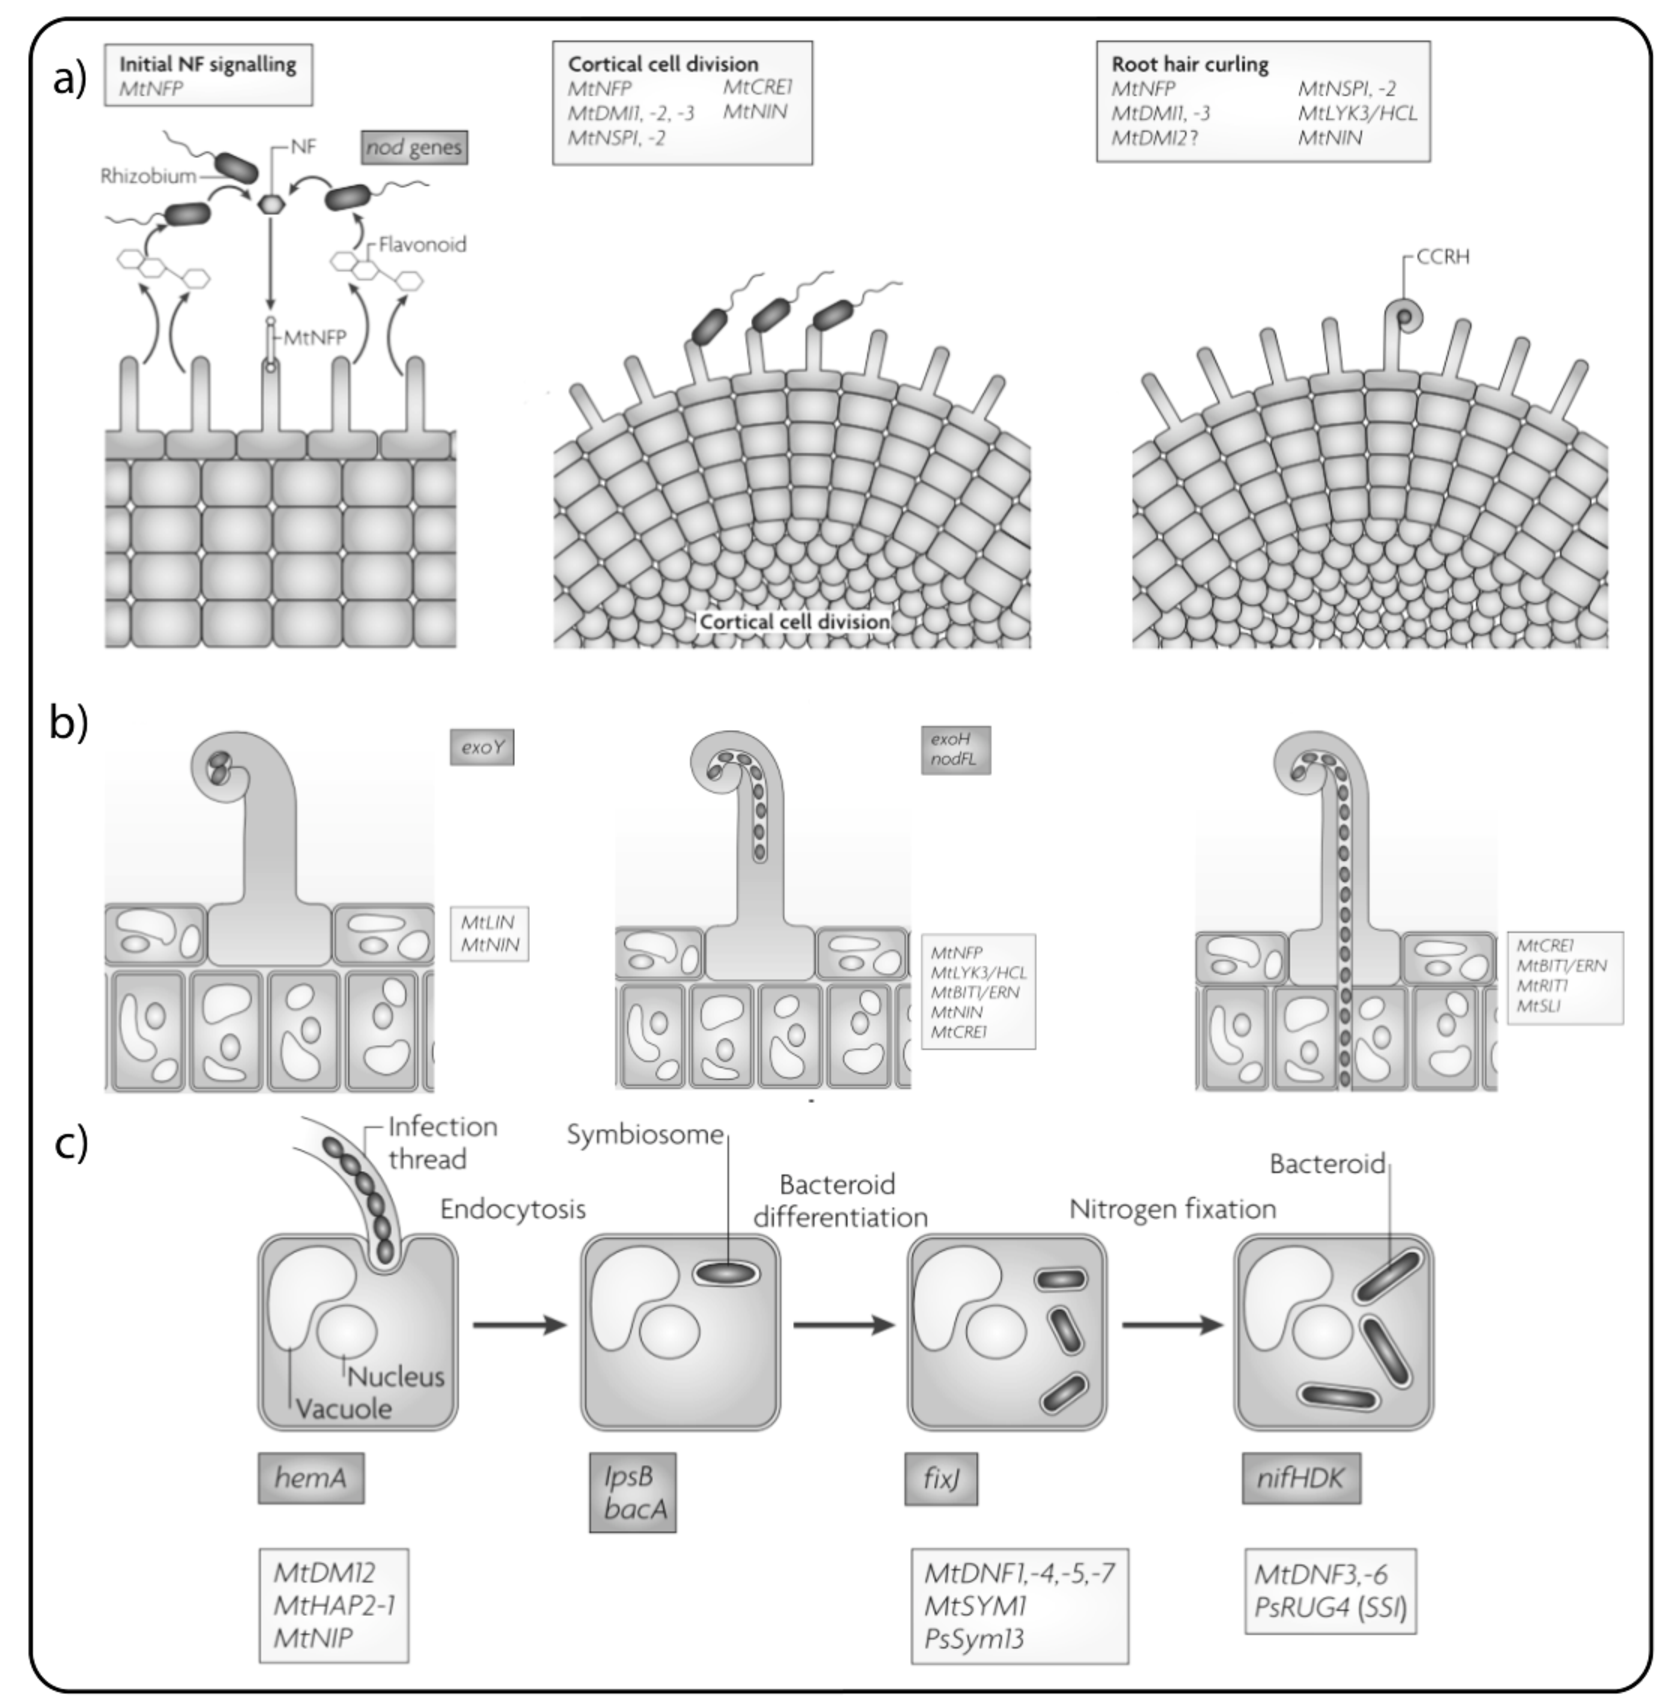
\includegraphics[width=1\textwidth]{figures/Introduction/thesis_17}
	\caption{\label{fig:symbiosis}\textbf{Details on the physiology and genetics of the \textit{S. meliloti} - \textit{M. sativa} symbiosis}\\
			a) Plant - bacteria recognition and adhesion\\
			b) Invasion and infection thread formation\\
			c) Bacteroid differentiation and nitrogen fixation\\
			Adapted from \cite{jones2007rhizobial}}
\end{figure}

%\subsubsection{Agricultural, economic and social impact of BNF}
%Big impact!
%\subsection{The role of the microbial community in the rhizosphere}
%A big role my friend!
%\subsection{Endophytes vs. symbionts}
%A big match!
\subsubsection{Host recognition, invasion and nodule formation}
The first step in the establishment of the symbiosis is the recognition between the plant and the bacterial cells in the rhizosphere: rhizobia sense the root exudates and move chemotaxically towards the roots surface \cite{barbour1991chemotaxis}\cite{caetano1992growth}; in particular, the plant signals recognized by the rhizobia are flavonoids, which are aromatic compounds with a 15 carbon skeleton, produced by the secondary metabolism of the plant. The flavonoids penetrate inside the rhizobial cells, where they are recognized by NodD, the master regulator of the \textit{nod} genes (Table \ref{tab:bnfgenes}), which lead to the production of the so-called \textit{nod factor}, a lipochito-oligosaccharide that is released from the rhizobia and that is recognized by the plant root, and stimulates the production of root hairs that will favour the invasion by the rhizobial cells \cite{shaw2006perception} (Figure \ref{fig:symbiosis}a). The chemical composition of the nod factor is highly specific, precisely determining the so-called host range of the rhizobial species, that are the plant species that recognize that particular nod factor and allow the invasion \cite{kondorosi1984physical}.

\begin{table}
    \begin{tabularx}{\textwidth}{|p{4cm}|p{8.2cm}|}
        \hline
        Gene group              & Function                                                                         \\ \hline
        Common \textit{nod} genes        & Synthesis of the general structure of the nod factor                             \\ 
        Host-specific \textit{nod} genes & Generally not conserved across rhizobial species, determine the host specificity \\ 
        \textit{nif} genes               & Synthesis, regulation and operation of the nitrogen fixation process             \\ 
        \textit{fix} genes               & Regulation of the nitrogen fixation process inside the nodule environment        \\
        \hline
    \end{tabularx}
	\caption{\label{tab:bnfgenes}\textbf{Main genes involved in the establishment of the rhizobia - leguminous plants symbiosis}}
\end{table}

Once that the rhizobial cells adhere to the root hair, thanks to the surface lectins produced by the plant, the local production of nod factor induce a local growth of the root hair, causing a curled development that traps the rhizobial cells on the root hair tip \cite{diaz1986correlation}. An hydrolysis on the plant cells wall leads then to the formation of the so-called \textit{infection thread}, a tubular growth of the rhizobial cells along the root hair (Figure \ref{fig:symbiosis}b).

When the infection thread reaches the base of the root hair, the rhizobial cells are internalized by the bark cells and are included by endocytosis in vescicles termed \textit{symbiosomes}, where they undergo a series of physiological changes to a form termed \textit{bacteroid} \cite{brewin2004plant}, while the plant root cells are growing, leading to the formation of the nodule, an oval organ attacched to the root. Depending on the shape and internal physiology of the nodule, they can be divided in two groups, \textit{determined} and \textit{indetermined}, with the latter being typical to the \textit{Sinorhizobium} - \textit{Medicago} symbiosis (Figure \ref{fig:symbiosis}c).

\begin{itemize}
\item \textbf{Determined nodules:} this nodules are typical of tropical and subtropical legumes, are characterized by a globolose shape, the absence of a meristematic activity; bacteroid found in this nodules are comparable to free living cells in terms of DNA content, cell shape and size and viability \cite{brewin1991development}\cite{franssen1992developmental}\cite{mergaert2006eukaryotic}.
\item \textbf{Indetermined nodules:} this nodules, typical of temperate legumes, have a more elongated shape (caused by a persistent meristematic activity) and with the internal rhizobial cells showing a distinct degree in differentiation in bacteroids (with five distinct differentiation steps) in the various zones of the nodule (four distinct zones) \cite{patriarca2002key}\cite{pawlowski1996rhizobial}\cite{vasse1990correlation}.
\end{itemize}

The bacteroids found in indeterminate nodules are bigger in size, more elongated and with an increased DNA content, with multiple nucleoids; the cells viability is highly reduced when rhizobial cells are in this state, most probably because of serious impairs in the cell cycle \cite{mergaert2006eukaryotic}.

\subsubsection{Nitrogen fixation}
The process of BNF is mediated through the enzyme nitrogenase, which converts the inert atmospheric nitrogen (N\textsubscript{2}) to the accessible form of ammonia (NH\textsubscript{3}) \cite{peters2006exploring}; this enzyme is present in prokaryotes (the groups \textit{Rhizobia}, \textit{Cyanobacteria}, \textit{Azobacteria}, the genus \textit{Frankia}) and some \textit{Archaea} \cite{raymond2004natural}. In the \textit{Sinorhizobium} - \textit{Medicago} symbiosis, the nitrogen fixation takes place inside the nodules symbiosomes by the differentiated bacteroids, which exhibit a significant downregulation of many metabolic functions, together with an upregulation of the genes related to nitrogenase activity \cite{barnett2006global}; this particular enzymatic  activity needs a considerable amount of energy, with 16 ATP molecules needed to fix a single molecule of atmospheric nitrogen \cite{poole2000carbon}, energy that is provided by the plant, in the form of photosynthesis products in return of the fixed ammonia \cite{lodwig2003metabolism}. Another key factor for an efficient BNF is the O\textsubscript{2} concentration, which inhibits the nitrogenase activity, but it is also needed for cellular respiration: the modulation of the oxygen concentration inside the nodule is therefore critical for the overall BNF process; this regulation is performed thanks to the leghaemoglobin, which is constituted by an heme produced by the rhizobial cells and a globinic part provided by the plant \cite{o1987bacterial}. The presence of the leghemoglobin confers the typical light-red color of the nodules in which active nitrogen fixation is carried on (Figure \ref{fig:nodules}).

\begin{figure}[!tb]
	\center
    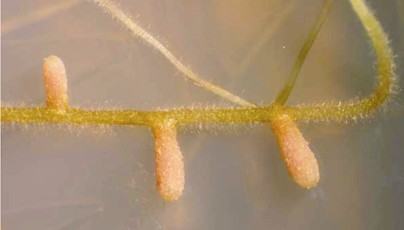
\includegraphics[width=0.66\textwidth]{figures/Introduction/thesis_18}
	\caption{\label{fig:nodules}\textbf{Nodules with active BNF}\\
			Indeterminate nodules exhibiting the typical light-red color of active nitrogen fixation, from a \textit{Sinorhizobium} - \textit{Medicago} nodulation experiment}
\end{figure}

\subsubsection{Genomics of symbiosis in \textit{S. meliloti}}
\label{sec:genomicsmeliloti}
Given the agricultural, economical and environmental importance of the \textit{Sinorhizobium} - \textit{Medicago} symbiosis, a considerable effort has been put towards the understanding of the genetic basis of this symbiosis: thanks to the technological advances in bacterial genomics, the first complete genomic sequence of a \textit{Sinorhizobium meliloti} strain was obtained in 2001 \cite{galibert2001composite}. The genome of this species is considerably bigger than many other bacteria, with 6.7 Mb (E. coli has a genome of about 4.5 Mb) and a peculiar multipartite structure, harboring a chromosome (3.65 Mb) and two megaplasmids termed pSymA (1.35 Mb) and pSymB (1.68 Mb); the presence of housekeeping functions on the latter megaplasmid has lead to its recent redefinition as a \textit{chromid}, that are megaplasmids with comparable GC content to the main chromosome and harboring essential genes \cite{harrison2010introducing}. The relative large genome of S. meliloti, together with the high number of paralogs and duplicated regions is consistent with the life-style of this species, since it needs to perform an efficient nitrogen fixation to avoid plant sanctions \cite{denison2004most}, and because of the competition inside the rhizosphere and in soil. An interesting genetical and evolutionary feature of this multipartite genome it's the different functional signature of each replicon, with most of the house-keeping genes present in the chromosome, most of the small molecules transporters belonging to pSymB and the vast majority of the genes needed for symbiosis, (including various duplicated copies) and nitrogen metabolism (\textit{nos}, \textit{nor}, and \textit{nap}) belonging to pSymA, whose codon usage and GC content supports the thesis of its origin by horizontal gene transfer events. There are also evidences of a spacial localization of some key symbiotic genes located on the pSymA replicon, with a particular focus on genes expressed in the bacteroid form and in microoxic conditions \cite{becker2004global} (Figure \ref{fig:spacial}), a feature that supports the thesis of an HGT origin of the symbiotic cluster. 

\begin{figure}[!tb]
	\center
    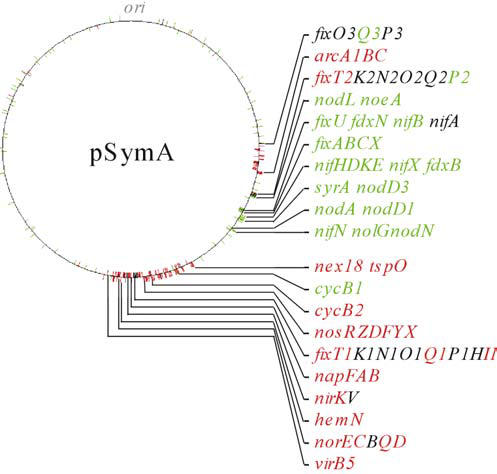
\includegraphics[width=0.6\textwidth]{figures/Introduction/thesis_19}
	\caption{\label{fig:spacial}\textbf{Spacial organization of key symbiotic genes on the pSymA megaplasmid}\\
			Position of genes induced in microoxic conditions (red), of genes induced in bacteroids (green) and in both conditions (black) (from \cite{becker2004global})}
\end{figure}

\subsubsection{Natural variability of \textit{S. meliloti}}
The genomic analysis on the \textit{Sinorhizobium meliloti} Rm1021 strain has been an important landmark in the understanding of the symbiotic process; however there are still some aspects of the \textit{Sinorhizobium} - \textit{Medicago} symbiosis that need to be studied, in order to optimize this process and extend it to a more rational use for the growing need of the modern world. A key point that needs to be addressed is the extent and the genetic origin of the natural diversity in the various aspects of the plant growth promotion phenotype, including the increase in plant growth, the resistance to specific environmental stresses like high salt concentration and host specificity; understanding the evolutionary dynamics of the composite genome is also an interesting issue, since it may shed some light on the origin of the symbiotic genes and to what extent they are conserved inside rhizobia. The final goal of such studies would be the definition of a series of genetic elements that are correlated with desirable plant growth promoting phenotypes, that can be then used with genetic engineering approaches towards the design of new strains of \textit{Sinorhizobium meliloti}. Some studies using CGH arrays have already established that there is indeed a certain degree of genetic diversity between different strains of \textit{S. meliloti}, exhibiting differences in the plant growth promoting ability \cite{giuntini2005large}: about 5\% of the genes of the Rm1021 strain showed signs of genetic variability in four natural strains, with the majority of this mutations occurring on the megaplasmid pSymA, suggesting an important role of this replicon in explaining the observed phenotypic variability.

%%-----------
%% Backmatter
%%-----------
\backmatter
\chaptermark{Bibliography}
\renewcommand{\sectionmark}[1]{\markright{#1}}
\bibliographystyle{unsrt}                           %Use alpha codes for references
\sectionmark{Bibliography}
\addcontentsline{toc}{chapter}{Bibliography}        %Force addition of Bibliography to TOC    
\bibliography{References}